\documentclass{article}
% \usepackage{covergraphic}
\usepackage{graphicx}
\usepackage{ragged2e}
\usepackage{xcolor}
\colorlet{coverdarkcolor}{black}
\definecolor{coverbgcolor}{RGB}{212,175,55}  % gold
\definecolor{coverboldcolor}{RGB}{0,67,37}  % green
% \definecolor{coverboldcolor}{RGB}{103,0,153}  % purple

\usepackage[defaultsans]{lato}

\usepackage{stackengine}
\renewcommand{\stackalignment}{c}

% I want the booleans offered by this package
\usepackage{etoolbox}
% Guidelines help to arrange the parts visually.  Show or not?
\newbool{showguidelinesbool}
  % set the default by uncommenting one or the other
  % \booltrue{showguidelinesbool} 
  \boolfalse{showguidelinesbool}  
% You can cause guidelines to be shown by invoking with
%   pdflatex "\def\showguidelines{}\documentclass{article}
% \usepackage{covergraphic}
\usepackage{graphicx}
\usepackage{ragged2e}
\usepackage{xcolor}
\colorlet{coverdarkcolor}{black}
\definecolor{coverbgcolor}{RGB}{212,175,55}  % gold
\definecolor{coverboldcolor}{RGB}{0,67,37}  % green
% \definecolor{coverboldcolor}{RGB}{103,0,153}  % purple

\usepackage[defaultsans]{lato}

\usepackage{stackengine}
\renewcommand{\stackalignment}{c}

% I want the booleans offered by this package
\usepackage{etoolbox}
% Guidelines help to arrange the parts visually.  Show or not?
\newbool{showguidelinesbool}
  % set the default by uncommenting one or the other
  % \booltrue{showguidelinesbool} 
  \boolfalse{showguidelinesbool}  
% You can cause guidelines to be shown by invoking with
%   pdflatex "\def\showguidelines{}\documentclass{article}
% \usepackage{covergraphic}
\usepackage{graphicx}
\usepackage{ragged2e}
\usepackage{xcolor}
\colorlet{coverdarkcolor}{black}
\definecolor{coverbgcolor}{RGB}{212,175,55}  % gold
\definecolor{coverboldcolor}{RGB}{0,67,37}  % green
% \definecolor{coverboldcolor}{RGB}{103,0,153}  % purple

\usepackage[defaultsans]{lato}

\usepackage{stackengine}
\renewcommand{\stackalignment}{c}

% I want the booleans offered by this package
\usepackage{etoolbox}
% Guidelines help to arrange the parts visually.  Show or not?
\newbool{showguidelinesbool}
  % set the default by uncommenting one or the other
  % \booltrue{showguidelinesbool} 
  \boolfalse{showguidelinesbool}  
% You can cause guidelines to be shown by invoking with
%   pdflatex "\def\showguidelines{}\documentclass{article}
% \usepackage{covergraphic}
\usepackage{graphicx}
\usepackage{ragged2e}
\usepackage{xcolor}
\colorlet{coverdarkcolor}{black}
\definecolor{coverbgcolor}{RGB}{212,175,55}  % gold
\definecolor{coverboldcolor}{RGB}{0,67,37}  % green
% \definecolor{coverboldcolor}{RGB}{103,0,153}  % purple

\usepackage[defaultsans]{lato}

\usepackage{stackengine}
\renewcommand{\stackalignment}{c}

% I want the booleans offered by this package
\usepackage{etoolbox}
% Guidelines help to arrange the parts visually.  Show or not?
\newbool{showguidelinesbool}
  % set the default by uncommenting one or the other
  % \booltrue{showguidelinesbool} 
  \boolfalse{showguidelinesbool}  
% You can cause guidelines to be shown by invoking with
%   pdflatex "\def\showguidelines{}\input{cover}"
% See http://stackoverflow.com/a/1466610
\ifdefined\showguidelines
  \booltrue{showguidelinesbool}
\fi
\ifbool{showguidelinesbool}{\typeout{!!! GUIDELINES SHOWN}}{}
% Guidelines to show KDP lines.  Show or not?
\newbool{showkdplinesbool}
  % set the default by uncommenting one or the other
  \booltrue{showkdplinesbool} 
  % \boolfalse{showkdplinesbool}  
% You can cause KDP lines to be shown by invoking with
%   pdflatex "\def\showkdplines{}\input{cover}"
\ifdefined\showkdplines
  \booltrue{showkdplinesbool}
\fi
\ifbool{showkdplinesbool}{\typeout{!!! KDP LINES SHOWN}}{}

% Size of page
% Kindle Direct Publishing gives this for a 531 page book;
% see the graphic KDP_diagram_531_pages.png
% # 	Description 	Width (in) 	Height (in)
% 1 	Full Cover 	16.446 	9.5
% 2 	Front Cover 	7.5 	9.25
% 3 	Safe Area 	7.375 	9
% 4 	Bleed 	0.125 	0.125
% 5 	Margin 	0.125 	0.125
% 6 	Spine 	1.196 	9.25
% 7 	Spine Safe Area 	1.071 	9
% 8 	Spine Margin 	0.062 	0.062
% 9 	Barcode Margin 	0.25 	0.25 

% I could calculate some of these from the others, but why?
% Number 3
\newlength{\FrontCoverSafeWidth}
  \setlength{\FrontCoverSafeWidth}{7.375in}
\newlength{\FrontCoverSafeHeight}
  \setlength{\FrontCoverSafeHeight}{9in}
% Number 5
\newlength{\FrontCoverMarginWidth}
  \setlength{\FrontCoverMarginWidth}{0.125in}
\newlength{\FrontCoverMarginHeight}
  \setlength{\FrontCoverMarginHeight}{0.125in}
% Number 2
\newlength{\FrontCoverWidth}
  \setlength{\FrontCoverWidth}{7.5in}
\newlength{\FrontCoverHeight}
  \setlength{\FrontCoverHeight}{9.25in}
% Number 4
\newlength{\BleedWidth}
  \setlength{\BleedWidth}{0.125in}
\newlength{\BleedHeight}
  \setlength{\BleedHeight}{0.125in}
% Number 7
\newlength{\SpineSafeWidth}
  \setlength{\SpineSafeWidth}{1.071in}
\newlength{\SpineSafeHeight}
  \setlength{\SpineSafeHeight}{9.0in}
% Number 8
\newlength{\SpineMarginWidth}
  \setlength{\SpineMarginWidth}{0.062in}
\newlength{\SpineMarginHeight}
  \setlength{\SpineMarginHeight}{0.062in}
% Number 9
\newlength{\BarcodeMarginWidth}
  \setlength{\BarcodeMarginWidth}{0.25in}
\newlength{\BarcodeMarginHeight}
  \setlength{\BarcodeMarginHeight}{0.25in}
% Number 6
\newlength{\SpineWidth}
  \setlength{\SpineWidth}{7.375in}
\newlength{\SpineHeight}
  \setlength{\SpineHeight}{9in}
% Number 1
\newlength{\FullCoverWidth}
  \setlength{\FullCoverWidth}{16.446in}
\newlength{\FullCoverHeight}
  \setlength{\FullCoverHeight}{9.5in}

\newlength{\totalcoverwidth} \setlength{\totalcoverwidth}{15.0in} % 7.5+7.5
\newlength{\spinewidth} \setlength{\spinewidth}{1in}
\addtolength{\totalcoverwidth}{\spinewidth}
\usepackage[papersize={16.446in,10in},margin=0in]{geometry}  

% ==== Spine ========
% 
\newcommand{\spinetext}[1]{\color{black}\fontsize{38pt}{8pt}{\fontfamily{ugq}\selectfont #1}}
\newcommand{\spineauthortext}[1]{\color{coverdarkcolor}\fontsize{23pt}{8pt}{\fontfamily{ugq}\selectfont{#1}}}
\newcommand{\spine}{%
\setlength{\unitlength}{1in}
\begin{picture}(1,9.5)
  \setstackgap{S}{2.1ex}
  % \put(0.235,5.65){\Shortstack{{\spinetext{L}} {\spinetext{I}} {\spinetext{N}} {\spinetext{E}} {\spinetext{A}} {\spinetext{R}}}}
  \put(0.18,8.5){\rotatebox[origin=lc]{-90}{\spinetext{Linear Algebra}\hspace{2.15in}\spineauthortext{Hef{}feron}}}
  \setstackgap{S}{0.9ex}
  % \put(0.3925,1.15){\Shortstack{{\spineauthortext{H}{14}} {\spineauthortext{E}{14}} {\spineauthortext{F}{14}} {\spineauthortext{F}{14}} {\spineauthortext{E}{14}} {\spineauthortext{R}{14}} {\spineauthortext{O}{14}} {\spineauthortext{N}{14}}}} % tried fake small caps by making the H be 14 pt, others be 11
\end{picture}
}


% ==== Back cover ========
% 
\newcommand{\backcovertext}{%
\RaggedRight
\color{black}\fontsize{14pt}{17pt}\fontfamily{fos}\selectfont
\begin{minipage}[t]{5.75in}
\setlength{\parskip}{1.4ex}
This text covers a standard first course:
Gauss's Method, vector spaces, linear maps and matrices, determinants,
and eigenvalues and eigenvectors.
In addition, each chapter ends with some
brief topics, including applications.

What sets this book apart is careful motivation, 
many examples, and extensive exercise sets.
Together, these help each student master the material of
the course and also help an instructor develop their student's  
level of mathematical maturity.

This book
has been freely available online for many years. 
It is widely used, 
both in classrooms and for self-study.
It is supported by worked answers for all exercises, 
projection slides for classroom use, 
and a lab manual based on \textit{Sage}. 

\vspace{.2in}
\noindent\textbf{Winner of the Math Association of America's Solow Award:}\\[1.35ex]
\vspace{-.225in}
\begin{center}
\parbox{5.5in}{
``The clear writing style, tremendous variety of exercises,
amenability to use with active learning strategies, and the
careful attention to detail in preparation mean that the text
is exceptionally adaptable.''}
\end{center}
\end{minipage}
}

\newcommand{\backcoverhead}{%
\setlength{\unitlength}{1in}
\begin{picture}(0,0)
  % \put(1,-.1){{\color{coverbgcolor}\rule{4.4in}{2pt}}}
  \put(0,-.1){{\color{coverbgcolor}\rule{5.05in}{2pt}}}
  \put(0.0,0){\color{coverboldcolor}\fontsize{25pt}{8pt}\fontfamily{fos}\selectfont \textit{A developmental approach to}}
  \put(3.0,-.45){\color{black}\fontsize{25pt}{8pt}\fontfamily{fos}\selectfont \textbf{Linear Algebra}}
\end{picture}
}




% ==== Front cover ========
% 
\newcommand{\frontcovertext}[1]{\color{black}\fontsize{55pt}{8pt}{\fontfamily{ugq}\selectfont #1}}
% \newcommand{\frontcovereditiontext}[1]{\color{black}\fontsize{20pt}{8pt}{\fontfamily{ugq}\selectfont #1}}
\newcommand{\frontcovereditiontext}[1]{\color[gray]{0.4}\fontsize{20pt}{6pt}\fontfamily{ugq}\selectfont \textsf{#1}}
% \newcommand{\frontcovereditiontext}[1]{\color{black}\fontsize{20pt}{6pt}\fontfamily{ugq}\selectfont #1}
\newcommand{\frontcoverauthortext}[1]{\color{black}\fontsize{27.5pt}{6pt}{\fontfamily{ugq}\selectfont #1}}
\newcommand{\frontcoverurltext}[1]{\color[gray]{0.4}\fontsize{18pt}{6pt}\fontfamily{ugq}\selectfont \textsf{#1}}
% \newcommand{\frontcoverurltext}[1]{\color[gray]{0.4}{\lato \fontsize{18pt}{6pt}\fontseries{sb}\selectfont #1}}


\setlength{\parindent}{0in}
\begin{document}\pagestyle{empty}\thispagestyle{empty}

\setlength{\unitlength}{1in}
\begin{picture}(0,0) 
  \ifbool{showguidelinesbool}{% 
    \put(0,-1){\makebox[0in]{\color{red}0}}
    \put(1,-1){\makebox[0in]{\color{red}1}}
    \put(2,-1){\makebox[0in]{\color{red}2}}
    \put(3,-1){\makebox[0in]{\color{red}3}}
    \put(4,-1){\makebox[0in]{\color{red}4}}
    \put(5,-1){\makebox[0in]{\color{red}5}}
    \put(6,-1){\makebox[0in]{\color{red}6}}
    \put(7,-1){\makebox[0in]{\color{red}7}}
    \put(7.5,-1){\color{red}\line(0,-1){8}}
    \put(8,-1){\makebox[0in]{\color{red}8}}
    \put(8,-1){\color{blue}\line(0,-1){8}}
    \put(8.5,-1){\color{red}\line(0,-1){8}}
    \put(9,-1){\makebox[0in]{\color{red}9}}
    \put(9.5,-1){\color{blue}\line(0,-1){8}}
    \put(10,-1){\makebox[0in]{\color{red}10}}
    \put(11,-1){\makebox[0in]{\color{red}11}}
    \put(12,-1){\makebox[0in]{\color{red}12}}
    \put(13,-1){\makebox[0in]{\color{red}13}}
    \put(14,-1){\makebox[0in]{\color{red}14}}
    \put(15,-1){\makebox[0in]{\color{red}15}}
    \put(15,-1){\color{blue}\line(0,-1){8}}
    \put(16,-1){\makebox[0in]{\color{red}16}}
  }{} 

  \put(9.5,-7.57){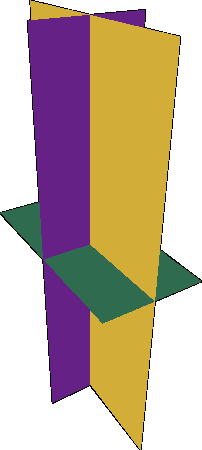
\includegraphics{asy/axesgraphic.pdf}}
  \put(9.5,-8.5){
\includegraphics{asy/shadow.pdf}}
  \put(15.25,-3){\makebox[0pt][r]{\frontcovertext{Linear Algebra}}}
  \put(15.25,-3.7){\makebox[0pt][r]{\frontcoverauthortext{Jim Hef{}feron}}}
  \put(15.25,-7.95){\makebox[0pt][r]{\frontcoverurltext{hefferon.net/linearalgebra}}}
  \put(15.25,-2.20){\makebox[0pt][r]{\frontcovereditiontext{Fourth edition}}}
  \put(7.65,-9.5){\spine}
  \put(1.0,-1.0){\backcoverhead}
  \put(1.0,-1.9){\backcovertext}

  \ifbool{showkdplinesbool}{% 
    % Front Cover width, height
    % Back cover
    \put(0.125,-0.125){\color{blue}\line(1,0){7.5}} % \FrontCoverWidth wide
      \put(0.125,-9.375){\color{blue}\line(1,0){7.5}} % \FrontCoverWidth wide
      \put(0.125,-0.125){\color{blue}\line(0,-1){9.25}} % \FrontCoverHeight tall
      \put(7.625,-0.125){\color{blue}\line(0,-1){9.25}}
    \put(0.25,-0.25){\color{blue}\line(1,0){7.375}} % \FrontCoverSafeWidth wide
      \put(0.25,-9.25){\color{blue}\line(1,0){7.375}} % \FrontCoverSafeWidth wide
      \put(0.25,-0.25){\color{blue}\line(0,-1){9.0}} % \FrontCoverSafeHeight tall
    % % Spine
    \put(7.687,-0.25){\color{blue}\line(1,0){1.071}} % 
      \put(7.687,-9.25){\color{blue}\line(1,0){1.071}} % 
    \put(7.687,-0.25){\color{blue}\line(0,-1){9}} %
      \put(8.758,-0.25){\color{blue}\line(0,-1){9}} %
    % % Front Cover
    \put(16.341,-0.125){\color{blue}\line(-1,0){7.5}} % 
      \put(16.341,-9.375){\color{blue}\line(-1,0){7.5}} % 
    \put(16.341,-0.125){\color{blue}\line(0,-1){9.25}} % 
      \put(8.821,-0.125){\color{blue}\line(0,-1){9.25}} % 
    \put(16.216,-0.25){\color{blue}\line(-1,0){7.375}} % Safe area
      \put(16.216,-9.25){\color{blue}\line(-1,0){7.375}} % 
    \put(16.216,-0.25){\color{blue}\line(0,-1){9}} % 
  }{}
\end{picture}
\end{document}
"
% See http://stackoverflow.com/a/1466610
\ifdefined\showguidelines
  \booltrue{showguidelinesbool}
\fi
\ifbool{showguidelinesbool}{\typeout{!!! GUIDELINES SHOWN}}{}
% Guidelines to show KDP lines.  Show or not?
\newbool{showkdplinesbool}
  % set the default by uncommenting one or the other
  \booltrue{showkdplinesbool} 
  % \boolfalse{showkdplinesbool}  
% You can cause KDP lines to be shown by invoking with
%   pdflatex "\def\showkdplines{}\documentclass{article}
% \usepackage{covergraphic}
\usepackage{graphicx}
\usepackage{ragged2e}
\usepackage{xcolor}
\colorlet{coverdarkcolor}{black}
\definecolor{coverbgcolor}{RGB}{212,175,55}  % gold
\definecolor{coverboldcolor}{RGB}{0,67,37}  % green
% \definecolor{coverboldcolor}{RGB}{103,0,153}  % purple

\usepackage[defaultsans]{lato}

\usepackage{stackengine}
\renewcommand{\stackalignment}{c}

% I want the booleans offered by this package
\usepackage{etoolbox}
% Guidelines help to arrange the parts visually.  Show or not?
\newbool{showguidelinesbool}
  % set the default by uncommenting one or the other
  % \booltrue{showguidelinesbool} 
  \boolfalse{showguidelinesbool}  
% You can cause guidelines to be shown by invoking with
%   pdflatex "\def\showguidelines{}\input{cover}"
% See http://stackoverflow.com/a/1466610
\ifdefined\showguidelines
  \booltrue{showguidelinesbool}
\fi
\ifbool{showguidelinesbool}{\typeout{!!! GUIDELINES SHOWN}}{}
% Guidelines to show KDP lines.  Show or not?
\newbool{showkdplinesbool}
  % set the default by uncommenting one or the other
  \booltrue{showkdplinesbool} 
  % \boolfalse{showkdplinesbool}  
% You can cause KDP lines to be shown by invoking with
%   pdflatex "\def\showkdplines{}\input{cover}"
\ifdefined\showkdplines
  \booltrue{showkdplinesbool}
\fi
\ifbool{showkdplinesbool}{\typeout{!!! KDP LINES SHOWN}}{}

% Size of page
% Kindle Direct Publishing gives this for a 531 page book;
% see the graphic KDP_diagram_531_pages.png
% # 	Description 	Width (in) 	Height (in)
% 1 	Full Cover 	16.446 	9.5
% 2 	Front Cover 	7.5 	9.25
% 3 	Safe Area 	7.375 	9
% 4 	Bleed 	0.125 	0.125
% 5 	Margin 	0.125 	0.125
% 6 	Spine 	1.196 	9.25
% 7 	Spine Safe Area 	1.071 	9
% 8 	Spine Margin 	0.062 	0.062
% 9 	Barcode Margin 	0.25 	0.25 

% I could calculate some of these from the others, but why?
% Number 3
\newlength{\FrontCoverSafeWidth}
  \setlength{\FrontCoverSafeWidth}{7.375in}
\newlength{\FrontCoverSafeHeight}
  \setlength{\FrontCoverSafeHeight}{9in}
% Number 5
\newlength{\FrontCoverMarginWidth}
  \setlength{\FrontCoverMarginWidth}{0.125in}
\newlength{\FrontCoverMarginHeight}
  \setlength{\FrontCoverMarginHeight}{0.125in}
% Number 2
\newlength{\FrontCoverWidth}
  \setlength{\FrontCoverWidth}{7.5in}
\newlength{\FrontCoverHeight}
  \setlength{\FrontCoverHeight}{9.25in}
% Number 4
\newlength{\BleedWidth}
  \setlength{\BleedWidth}{0.125in}
\newlength{\BleedHeight}
  \setlength{\BleedHeight}{0.125in}
% Number 7
\newlength{\SpineSafeWidth}
  \setlength{\SpineSafeWidth}{1.071in}
\newlength{\SpineSafeHeight}
  \setlength{\SpineSafeHeight}{9.0in}
% Number 8
\newlength{\SpineMarginWidth}
  \setlength{\SpineMarginWidth}{0.062in}
\newlength{\SpineMarginHeight}
  \setlength{\SpineMarginHeight}{0.062in}
% Number 9
\newlength{\BarcodeMarginWidth}
  \setlength{\BarcodeMarginWidth}{0.25in}
\newlength{\BarcodeMarginHeight}
  \setlength{\BarcodeMarginHeight}{0.25in}
% Number 6
\newlength{\SpineWidth}
  \setlength{\SpineWidth}{7.375in}
\newlength{\SpineHeight}
  \setlength{\SpineHeight}{9in}
% Number 1
\newlength{\FullCoverWidth}
  \setlength{\FullCoverWidth}{16.446in}
\newlength{\FullCoverHeight}
  \setlength{\FullCoverHeight}{9.5in}

\newlength{\totalcoverwidth} \setlength{\totalcoverwidth}{15.0in} % 7.5+7.5
\newlength{\spinewidth} \setlength{\spinewidth}{1in}
\addtolength{\totalcoverwidth}{\spinewidth}
\usepackage[papersize={16.446in,10in},margin=0in]{geometry}  

% ==== Spine ========
% 
\newcommand{\spinetext}[1]{\color{black}\fontsize{38pt}{8pt}{\fontfamily{ugq}\selectfont #1}}
\newcommand{\spineauthortext}[1]{\color{coverdarkcolor}\fontsize{23pt}{8pt}{\fontfamily{ugq}\selectfont{#1}}}
\newcommand{\spine}{%
\setlength{\unitlength}{1in}
\begin{picture}(1,9.5)
  \setstackgap{S}{2.1ex}
  % \put(0.235,5.65){\Shortstack{{\spinetext{L}} {\spinetext{I}} {\spinetext{N}} {\spinetext{E}} {\spinetext{A}} {\spinetext{R}}}}
  \put(0.18,8.5){\rotatebox[origin=lc]{-90}{\spinetext{Linear Algebra}\hspace{2.15in}\spineauthortext{Hef{}feron}}}
  \setstackgap{S}{0.9ex}
  % \put(0.3925,1.15){\Shortstack{{\spineauthortext{H}{14}} {\spineauthortext{E}{14}} {\spineauthortext{F}{14}} {\spineauthortext{F}{14}} {\spineauthortext{E}{14}} {\spineauthortext{R}{14}} {\spineauthortext{O}{14}} {\spineauthortext{N}{14}}}} % tried fake small caps by making the H be 14 pt, others be 11
\end{picture}
}


% ==== Back cover ========
% 
\newcommand{\backcovertext}{%
\RaggedRight
\color{black}\fontsize{14pt}{17pt}\fontfamily{fos}\selectfont
\begin{minipage}[t]{5.75in}
\setlength{\parskip}{1.4ex}
This text covers a standard first course:
Gauss's Method, vector spaces, linear maps and matrices, determinants,
and eigenvalues and eigenvectors.
In addition, each chapter ends with some
brief topics, including applications.

What sets this book apart is careful motivation, 
many examples, and extensive exercise sets.
Together, these help each student master the material of
the course and also help an instructor develop their student's  
level of mathematical maturity.

This book
has been freely available online for many years. 
It is widely used, 
both in classrooms and for self-study.
It is supported by worked answers for all exercises, 
projection slides for classroom use, 
and a lab manual based on \textit{Sage}. 

\vspace{.2in}
\noindent\textbf{Winner of the Math Association of America's Solow Award:}\\[1.35ex]
\vspace{-.225in}
\begin{center}
\parbox{5.5in}{
``The clear writing style, tremendous variety of exercises,
amenability to use with active learning strategies, and the
careful attention to detail in preparation mean that the text
is exceptionally adaptable.''}
\end{center}
\end{minipage}
}

\newcommand{\backcoverhead}{%
\setlength{\unitlength}{1in}
\begin{picture}(0,0)
  % \put(1,-.1){{\color{coverbgcolor}\rule{4.4in}{2pt}}}
  \put(0,-.1){{\color{coverbgcolor}\rule{5.05in}{2pt}}}
  \put(0.0,0){\color{coverboldcolor}\fontsize{25pt}{8pt}\fontfamily{fos}\selectfont \textit{A developmental approach to}}
  \put(3.0,-.45){\color{black}\fontsize{25pt}{8pt}\fontfamily{fos}\selectfont \textbf{Linear Algebra}}
\end{picture}
}




% ==== Front cover ========
% 
\newcommand{\frontcovertext}[1]{\color{black}\fontsize{55pt}{8pt}{\fontfamily{ugq}\selectfont #1}}
% \newcommand{\frontcovereditiontext}[1]{\color{black}\fontsize{20pt}{8pt}{\fontfamily{ugq}\selectfont #1}}
\newcommand{\frontcovereditiontext}[1]{\color[gray]{0.4}\fontsize{20pt}{6pt}\fontfamily{ugq}\selectfont \textsf{#1}}
% \newcommand{\frontcovereditiontext}[1]{\color{black}\fontsize{20pt}{6pt}\fontfamily{ugq}\selectfont #1}
\newcommand{\frontcoverauthortext}[1]{\color{black}\fontsize{27.5pt}{6pt}{\fontfamily{ugq}\selectfont #1}}
\newcommand{\frontcoverurltext}[1]{\color[gray]{0.4}\fontsize{18pt}{6pt}\fontfamily{ugq}\selectfont \textsf{#1}}
% \newcommand{\frontcoverurltext}[1]{\color[gray]{0.4}{\lato \fontsize{18pt}{6pt}\fontseries{sb}\selectfont #1}}


\setlength{\parindent}{0in}
\begin{document}\pagestyle{empty}\thispagestyle{empty}

\setlength{\unitlength}{1in}
\begin{picture}(0,0) 
  \ifbool{showguidelinesbool}{% 
    \put(0,-1){\makebox[0in]{\color{red}0}}
    \put(1,-1){\makebox[0in]{\color{red}1}}
    \put(2,-1){\makebox[0in]{\color{red}2}}
    \put(3,-1){\makebox[0in]{\color{red}3}}
    \put(4,-1){\makebox[0in]{\color{red}4}}
    \put(5,-1){\makebox[0in]{\color{red}5}}
    \put(6,-1){\makebox[0in]{\color{red}6}}
    \put(7,-1){\makebox[0in]{\color{red}7}}
    \put(7.5,-1){\color{red}\line(0,-1){8}}
    \put(8,-1){\makebox[0in]{\color{red}8}}
    \put(8,-1){\color{blue}\line(0,-1){8}}
    \put(8.5,-1){\color{red}\line(0,-1){8}}
    \put(9,-1){\makebox[0in]{\color{red}9}}
    \put(9.5,-1){\color{blue}\line(0,-1){8}}
    \put(10,-1){\makebox[0in]{\color{red}10}}
    \put(11,-1){\makebox[0in]{\color{red}11}}
    \put(12,-1){\makebox[0in]{\color{red}12}}
    \put(13,-1){\makebox[0in]{\color{red}13}}
    \put(14,-1){\makebox[0in]{\color{red}14}}
    \put(15,-1){\makebox[0in]{\color{red}15}}
    \put(15,-1){\color{blue}\line(0,-1){8}}
    \put(16,-1){\makebox[0in]{\color{red}16}}
  }{} 

  \put(9.5,-7.57){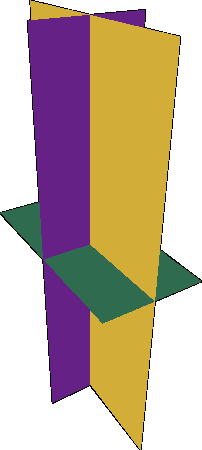
\includegraphics{asy/axesgraphic.pdf}}
  \put(9.5,-8.5){
\includegraphics{asy/shadow.pdf}}
  \put(15.25,-3){\makebox[0pt][r]{\frontcovertext{Linear Algebra}}}
  \put(15.25,-3.7){\makebox[0pt][r]{\frontcoverauthortext{Jim Hef{}feron}}}
  \put(15.25,-7.95){\makebox[0pt][r]{\frontcoverurltext{hefferon.net/linearalgebra}}}
  \put(15.25,-2.20){\makebox[0pt][r]{\frontcovereditiontext{Fourth edition}}}
  \put(7.65,-9.5){\spine}
  \put(1.0,-1.0){\backcoverhead}
  \put(1.0,-1.9){\backcovertext}

  \ifbool{showkdplinesbool}{% 
    % Front Cover width, height
    % Back cover
    \put(0.125,-0.125){\color{blue}\line(1,0){7.5}} % \FrontCoverWidth wide
      \put(0.125,-9.375){\color{blue}\line(1,0){7.5}} % \FrontCoverWidth wide
      \put(0.125,-0.125){\color{blue}\line(0,-1){9.25}} % \FrontCoverHeight tall
      \put(7.625,-0.125){\color{blue}\line(0,-1){9.25}}
    \put(0.25,-0.25){\color{blue}\line(1,0){7.375}} % \FrontCoverSafeWidth wide
      \put(0.25,-9.25){\color{blue}\line(1,0){7.375}} % \FrontCoverSafeWidth wide
      \put(0.25,-0.25){\color{blue}\line(0,-1){9.0}} % \FrontCoverSafeHeight tall
    % % Spine
    \put(7.687,-0.25){\color{blue}\line(1,0){1.071}} % 
      \put(7.687,-9.25){\color{blue}\line(1,0){1.071}} % 
    \put(7.687,-0.25){\color{blue}\line(0,-1){9}} %
      \put(8.758,-0.25){\color{blue}\line(0,-1){9}} %
    % % Front Cover
    \put(16.341,-0.125){\color{blue}\line(-1,0){7.5}} % 
      \put(16.341,-9.375){\color{blue}\line(-1,0){7.5}} % 
    \put(16.341,-0.125){\color{blue}\line(0,-1){9.25}} % 
      \put(8.821,-0.125){\color{blue}\line(0,-1){9.25}} % 
    \put(16.216,-0.25){\color{blue}\line(-1,0){7.375}} % Safe area
      \put(16.216,-9.25){\color{blue}\line(-1,0){7.375}} % 
    \put(16.216,-0.25){\color{blue}\line(0,-1){9}} % 
  }{}
\end{picture}
\end{document}
"
\ifdefined\showkdplines
  \booltrue{showkdplinesbool}
\fi
\ifbool{showkdplinesbool}{\typeout{!!! KDP LINES SHOWN}}{}

% Size of page
% Kindle Direct Publishing gives this for a 531 page book;
% see the graphic KDP_diagram_531_pages.png
% # 	Description 	Width (in) 	Height (in)
% 1 	Full Cover 	16.446 	9.5
% 2 	Front Cover 	7.5 	9.25
% 3 	Safe Area 	7.375 	9
% 4 	Bleed 	0.125 	0.125
% 5 	Margin 	0.125 	0.125
% 6 	Spine 	1.196 	9.25
% 7 	Spine Safe Area 	1.071 	9
% 8 	Spine Margin 	0.062 	0.062
% 9 	Barcode Margin 	0.25 	0.25 

% I could calculate some of these from the others, but why?
% Number 3
\newlength{\FrontCoverSafeWidth}
  \setlength{\FrontCoverSafeWidth}{7.375in}
\newlength{\FrontCoverSafeHeight}
  \setlength{\FrontCoverSafeHeight}{9in}
% Number 5
\newlength{\FrontCoverMarginWidth}
  \setlength{\FrontCoverMarginWidth}{0.125in}
\newlength{\FrontCoverMarginHeight}
  \setlength{\FrontCoverMarginHeight}{0.125in}
% Number 2
\newlength{\FrontCoverWidth}
  \setlength{\FrontCoverWidth}{7.5in}
\newlength{\FrontCoverHeight}
  \setlength{\FrontCoverHeight}{9.25in}
% Number 4
\newlength{\BleedWidth}
  \setlength{\BleedWidth}{0.125in}
\newlength{\BleedHeight}
  \setlength{\BleedHeight}{0.125in}
% Number 7
\newlength{\SpineSafeWidth}
  \setlength{\SpineSafeWidth}{1.071in}
\newlength{\SpineSafeHeight}
  \setlength{\SpineSafeHeight}{9.0in}
% Number 8
\newlength{\SpineMarginWidth}
  \setlength{\SpineMarginWidth}{0.062in}
\newlength{\SpineMarginHeight}
  \setlength{\SpineMarginHeight}{0.062in}
% Number 9
\newlength{\BarcodeMarginWidth}
  \setlength{\BarcodeMarginWidth}{0.25in}
\newlength{\BarcodeMarginHeight}
  \setlength{\BarcodeMarginHeight}{0.25in}
% Number 6
\newlength{\SpineWidth}
  \setlength{\SpineWidth}{7.375in}
\newlength{\SpineHeight}
  \setlength{\SpineHeight}{9in}
% Number 1
\newlength{\FullCoverWidth}
  \setlength{\FullCoverWidth}{16.446in}
\newlength{\FullCoverHeight}
  \setlength{\FullCoverHeight}{9.5in}

\newlength{\totalcoverwidth} \setlength{\totalcoverwidth}{15.0in} % 7.5+7.5
\newlength{\spinewidth} \setlength{\spinewidth}{1in}
\addtolength{\totalcoverwidth}{\spinewidth}
\usepackage[papersize={16.446in,10in},margin=0in]{geometry}  

% ==== Spine ========
% 
\newcommand{\spinetext}[1]{\color{black}\fontsize{38pt}{8pt}{\fontfamily{ugq}\selectfont #1}}
\newcommand{\spineauthortext}[1]{\color{coverdarkcolor}\fontsize{23pt}{8pt}{\fontfamily{ugq}\selectfont{#1}}}
\newcommand{\spine}{%
\setlength{\unitlength}{1in}
\begin{picture}(1,9.5)
  \setstackgap{S}{2.1ex}
  % \put(0.235,5.65){\Shortstack{{\spinetext{L}} {\spinetext{I}} {\spinetext{N}} {\spinetext{E}} {\spinetext{A}} {\spinetext{R}}}}
  \put(0.18,8.5){\rotatebox[origin=lc]{-90}{\spinetext{Linear Algebra}\hspace{2.15in}\spineauthortext{Hef{}feron}}}
  \setstackgap{S}{0.9ex}
  % \put(0.3925,1.15){\Shortstack{{\spineauthortext{H}{14}} {\spineauthortext{E}{14}} {\spineauthortext{F}{14}} {\spineauthortext{F}{14}} {\spineauthortext{E}{14}} {\spineauthortext{R}{14}} {\spineauthortext{O}{14}} {\spineauthortext{N}{14}}}} % tried fake small caps by making the H be 14 pt, others be 11
\end{picture}
}


% ==== Back cover ========
% 
\newcommand{\backcovertext}{%
\RaggedRight
\color{black}\fontsize{14pt}{17pt}\fontfamily{fos}\selectfont
\begin{minipage}[t]{5.75in}
\setlength{\parskip}{1.4ex}
This text covers a standard first course:
Gauss's Method, vector spaces, linear maps and matrices, determinants,
and eigenvalues and eigenvectors.
In addition, each chapter ends with some
brief topics, including applications.

What sets this book apart is careful motivation, 
many examples, and extensive exercise sets.
Together, these help each student master the material of
the course and also help an instructor develop their student's  
level of mathematical maturity.

This book
has been freely available online for many years. 
It is widely used, 
both in classrooms and for self-study.
It is supported by worked answers for all exercises, 
projection slides for classroom use, 
and a lab manual based on \textit{Sage}. 

\vspace{.2in}
\noindent\textbf{Winner of the Math Association of America's Solow Award:}\\[1.35ex]
\vspace{-.225in}
\begin{center}
\parbox{5.5in}{
``The clear writing style, tremendous variety of exercises,
amenability to use with active learning strategies, and the
careful attention to detail in preparation mean that the text
is exceptionally adaptable.''}
\end{center}
\end{minipage}
}

\newcommand{\backcoverhead}{%
\setlength{\unitlength}{1in}
\begin{picture}(0,0)
  % \put(1,-.1){{\color{coverbgcolor}\rule{4.4in}{2pt}}}
  \put(0,-.1){{\color{coverbgcolor}\rule{5.05in}{2pt}}}
  \put(0.0,0){\color{coverboldcolor}\fontsize{25pt}{8pt}\fontfamily{fos}\selectfont \textit{A developmental approach to}}
  \put(3.0,-.45){\color{black}\fontsize{25pt}{8pt}\fontfamily{fos}\selectfont \textbf{Linear Algebra}}
\end{picture}
}




% ==== Front cover ========
% 
\newcommand{\frontcovertext}[1]{\color{black}\fontsize{55pt}{8pt}{\fontfamily{ugq}\selectfont #1}}
% \newcommand{\frontcovereditiontext}[1]{\color{black}\fontsize{20pt}{8pt}{\fontfamily{ugq}\selectfont #1}}
\newcommand{\frontcovereditiontext}[1]{\color[gray]{0.4}\fontsize{20pt}{6pt}\fontfamily{ugq}\selectfont \textsf{#1}}
% \newcommand{\frontcovereditiontext}[1]{\color{black}\fontsize{20pt}{6pt}\fontfamily{ugq}\selectfont #1}
\newcommand{\frontcoverauthortext}[1]{\color{black}\fontsize{27.5pt}{6pt}{\fontfamily{ugq}\selectfont #1}}
\newcommand{\frontcoverurltext}[1]{\color[gray]{0.4}\fontsize{18pt}{6pt}\fontfamily{ugq}\selectfont \textsf{#1}}
% \newcommand{\frontcoverurltext}[1]{\color[gray]{0.4}{\lato \fontsize{18pt}{6pt}\fontseries{sb}\selectfont #1}}


\setlength{\parindent}{0in}
\begin{document}\pagestyle{empty}\thispagestyle{empty}

\setlength{\unitlength}{1in}
\begin{picture}(0,0) 
  \ifbool{showguidelinesbool}{% 
    \put(0,-1){\makebox[0in]{\color{red}0}}
    \put(1,-1){\makebox[0in]{\color{red}1}}
    \put(2,-1){\makebox[0in]{\color{red}2}}
    \put(3,-1){\makebox[0in]{\color{red}3}}
    \put(4,-1){\makebox[0in]{\color{red}4}}
    \put(5,-1){\makebox[0in]{\color{red}5}}
    \put(6,-1){\makebox[0in]{\color{red}6}}
    \put(7,-1){\makebox[0in]{\color{red}7}}
    \put(7.5,-1){\color{red}\line(0,-1){8}}
    \put(8,-1){\makebox[0in]{\color{red}8}}
    \put(8,-1){\color{blue}\line(0,-1){8}}
    \put(8.5,-1){\color{red}\line(0,-1){8}}
    \put(9,-1){\makebox[0in]{\color{red}9}}
    \put(9.5,-1){\color{blue}\line(0,-1){8}}
    \put(10,-1){\makebox[0in]{\color{red}10}}
    \put(11,-1){\makebox[0in]{\color{red}11}}
    \put(12,-1){\makebox[0in]{\color{red}12}}
    \put(13,-1){\makebox[0in]{\color{red}13}}
    \put(14,-1){\makebox[0in]{\color{red}14}}
    \put(15,-1){\makebox[0in]{\color{red}15}}
    \put(15,-1){\color{blue}\line(0,-1){8}}
    \put(16,-1){\makebox[0in]{\color{red}16}}
  }{} 

  \put(9.5,-7.57){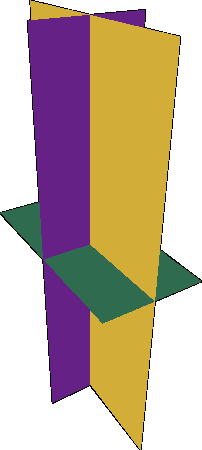
\includegraphics{asy/axesgraphic.pdf}}
  \put(9.5,-8.5){
\includegraphics{asy/shadow.pdf}}
  \put(15.25,-3){\makebox[0pt][r]{\frontcovertext{Linear Algebra}}}
  \put(15.25,-3.7){\makebox[0pt][r]{\frontcoverauthortext{Jim Hef{}feron}}}
  \put(15.25,-7.95){\makebox[0pt][r]{\frontcoverurltext{hefferon.net/linearalgebra}}}
  \put(15.25,-2.20){\makebox[0pt][r]{\frontcovereditiontext{Fourth edition}}}
  \put(7.65,-9.5){\spine}
  \put(1.0,-1.0){\backcoverhead}
  \put(1.0,-1.9){\backcovertext}

  \ifbool{showkdplinesbool}{% 
    % Front Cover width, height
    % Back cover
    \put(0.125,-0.125){\color{blue}\line(1,0){7.5}} % \FrontCoverWidth wide
      \put(0.125,-9.375){\color{blue}\line(1,0){7.5}} % \FrontCoverWidth wide
      \put(0.125,-0.125){\color{blue}\line(0,-1){9.25}} % \FrontCoverHeight tall
      \put(7.625,-0.125){\color{blue}\line(0,-1){9.25}}
    \put(0.25,-0.25){\color{blue}\line(1,0){7.375}} % \FrontCoverSafeWidth wide
      \put(0.25,-9.25){\color{blue}\line(1,0){7.375}} % \FrontCoverSafeWidth wide
      \put(0.25,-0.25){\color{blue}\line(0,-1){9.0}} % \FrontCoverSafeHeight tall
    % % Spine
    \put(7.687,-0.25){\color{blue}\line(1,0){1.071}} % 
      \put(7.687,-9.25){\color{blue}\line(1,0){1.071}} % 
    \put(7.687,-0.25){\color{blue}\line(0,-1){9}} %
      \put(8.758,-0.25){\color{blue}\line(0,-1){9}} %
    % % Front Cover
    \put(16.341,-0.125){\color{blue}\line(-1,0){7.5}} % 
      \put(16.341,-9.375){\color{blue}\line(-1,0){7.5}} % 
    \put(16.341,-0.125){\color{blue}\line(0,-1){9.25}} % 
      \put(8.821,-0.125){\color{blue}\line(0,-1){9.25}} % 
    \put(16.216,-0.25){\color{blue}\line(-1,0){7.375}} % Safe area
      \put(16.216,-9.25){\color{blue}\line(-1,0){7.375}} % 
    \put(16.216,-0.25){\color{blue}\line(0,-1){9}} % 
  }{}
\end{picture}
\end{document}
"
% See http://stackoverflow.com/a/1466610
\ifdefined\showguidelines
  \booltrue{showguidelinesbool}
\fi
\ifbool{showguidelinesbool}{\typeout{!!! GUIDELINES SHOWN}}{}
% Guidelines to show KDP lines.  Show or not?
\newbool{showkdplinesbool}
  % set the default by uncommenting one or the other
  \booltrue{showkdplinesbool} 
  % \boolfalse{showkdplinesbool}  
% You can cause KDP lines to be shown by invoking with
%   pdflatex "\def\showkdplines{}\documentclass{article}
% \usepackage{covergraphic}
\usepackage{graphicx}
\usepackage{ragged2e}
\usepackage{xcolor}
\colorlet{coverdarkcolor}{black}
\definecolor{coverbgcolor}{RGB}{212,175,55}  % gold
\definecolor{coverboldcolor}{RGB}{0,67,37}  % green
% \definecolor{coverboldcolor}{RGB}{103,0,153}  % purple

\usepackage[defaultsans]{lato}

\usepackage{stackengine}
\renewcommand{\stackalignment}{c}

% I want the booleans offered by this package
\usepackage{etoolbox}
% Guidelines help to arrange the parts visually.  Show or not?
\newbool{showguidelinesbool}
  % set the default by uncommenting one or the other
  % \booltrue{showguidelinesbool} 
  \boolfalse{showguidelinesbool}  
% You can cause guidelines to be shown by invoking with
%   pdflatex "\def\showguidelines{}\documentclass{article}
% \usepackage{covergraphic}
\usepackage{graphicx}
\usepackage{ragged2e}
\usepackage{xcolor}
\colorlet{coverdarkcolor}{black}
\definecolor{coverbgcolor}{RGB}{212,175,55}  % gold
\definecolor{coverboldcolor}{RGB}{0,67,37}  % green
% \definecolor{coverboldcolor}{RGB}{103,0,153}  % purple

\usepackage[defaultsans]{lato}

\usepackage{stackengine}
\renewcommand{\stackalignment}{c}

% I want the booleans offered by this package
\usepackage{etoolbox}
% Guidelines help to arrange the parts visually.  Show or not?
\newbool{showguidelinesbool}
  % set the default by uncommenting one or the other
  % \booltrue{showguidelinesbool} 
  \boolfalse{showguidelinesbool}  
% You can cause guidelines to be shown by invoking with
%   pdflatex "\def\showguidelines{}\input{cover}"
% See http://stackoverflow.com/a/1466610
\ifdefined\showguidelines
  \booltrue{showguidelinesbool}
\fi
\ifbool{showguidelinesbool}{\typeout{!!! GUIDELINES SHOWN}}{}
% Guidelines to show KDP lines.  Show or not?
\newbool{showkdplinesbool}
  % set the default by uncommenting one or the other
  \booltrue{showkdplinesbool} 
  % \boolfalse{showkdplinesbool}  
% You can cause KDP lines to be shown by invoking with
%   pdflatex "\def\showkdplines{}\input{cover}"
\ifdefined\showkdplines
  \booltrue{showkdplinesbool}
\fi
\ifbool{showkdplinesbool}{\typeout{!!! KDP LINES SHOWN}}{}

% Size of page
% Kindle Direct Publishing gives this for a 531 page book;
% see the graphic KDP_diagram_531_pages.png
% # 	Description 	Width (in) 	Height (in)
% 1 	Full Cover 	16.446 	9.5
% 2 	Front Cover 	7.5 	9.25
% 3 	Safe Area 	7.375 	9
% 4 	Bleed 	0.125 	0.125
% 5 	Margin 	0.125 	0.125
% 6 	Spine 	1.196 	9.25
% 7 	Spine Safe Area 	1.071 	9
% 8 	Spine Margin 	0.062 	0.062
% 9 	Barcode Margin 	0.25 	0.25 

% I could calculate some of these from the others, but why?
% Number 3
\newlength{\FrontCoverSafeWidth}
  \setlength{\FrontCoverSafeWidth}{7.375in}
\newlength{\FrontCoverSafeHeight}
  \setlength{\FrontCoverSafeHeight}{9in}
% Number 5
\newlength{\FrontCoverMarginWidth}
  \setlength{\FrontCoverMarginWidth}{0.125in}
\newlength{\FrontCoverMarginHeight}
  \setlength{\FrontCoverMarginHeight}{0.125in}
% Number 2
\newlength{\FrontCoverWidth}
  \setlength{\FrontCoverWidth}{7.5in}
\newlength{\FrontCoverHeight}
  \setlength{\FrontCoverHeight}{9.25in}
% Number 4
\newlength{\BleedWidth}
  \setlength{\BleedWidth}{0.125in}
\newlength{\BleedHeight}
  \setlength{\BleedHeight}{0.125in}
% Number 7
\newlength{\SpineSafeWidth}
  \setlength{\SpineSafeWidth}{1.071in}
\newlength{\SpineSafeHeight}
  \setlength{\SpineSafeHeight}{9.0in}
% Number 8
\newlength{\SpineMarginWidth}
  \setlength{\SpineMarginWidth}{0.062in}
\newlength{\SpineMarginHeight}
  \setlength{\SpineMarginHeight}{0.062in}
% Number 9
\newlength{\BarcodeMarginWidth}
  \setlength{\BarcodeMarginWidth}{0.25in}
\newlength{\BarcodeMarginHeight}
  \setlength{\BarcodeMarginHeight}{0.25in}
% Number 6
\newlength{\SpineWidth}
  \setlength{\SpineWidth}{7.375in}
\newlength{\SpineHeight}
  \setlength{\SpineHeight}{9in}
% Number 1
\newlength{\FullCoverWidth}
  \setlength{\FullCoverWidth}{16.446in}
\newlength{\FullCoverHeight}
  \setlength{\FullCoverHeight}{9.5in}

\newlength{\totalcoverwidth} \setlength{\totalcoverwidth}{15.0in} % 7.5+7.5
\newlength{\spinewidth} \setlength{\spinewidth}{1in}
\addtolength{\totalcoverwidth}{\spinewidth}
\usepackage[papersize={16.446in,10in},margin=0in]{geometry}  

% ==== Spine ========
% 
\newcommand{\spinetext}[1]{\color{black}\fontsize{38pt}{8pt}{\fontfamily{ugq}\selectfont #1}}
\newcommand{\spineauthortext}[1]{\color{coverdarkcolor}\fontsize{23pt}{8pt}{\fontfamily{ugq}\selectfont{#1}}}
\newcommand{\spine}{%
\setlength{\unitlength}{1in}
\begin{picture}(1,9.5)
  \setstackgap{S}{2.1ex}
  % \put(0.235,5.65){\Shortstack{{\spinetext{L}} {\spinetext{I}} {\spinetext{N}} {\spinetext{E}} {\spinetext{A}} {\spinetext{R}}}}
  \put(0.18,8.5){\rotatebox[origin=lc]{-90}{\spinetext{Linear Algebra}\hspace{2.15in}\spineauthortext{Hef{}feron}}}
  \setstackgap{S}{0.9ex}
  % \put(0.3925,1.15){\Shortstack{{\spineauthortext{H}{14}} {\spineauthortext{E}{14}} {\spineauthortext{F}{14}} {\spineauthortext{F}{14}} {\spineauthortext{E}{14}} {\spineauthortext{R}{14}} {\spineauthortext{O}{14}} {\spineauthortext{N}{14}}}} % tried fake small caps by making the H be 14 pt, others be 11
\end{picture}
}


% ==== Back cover ========
% 
\newcommand{\backcovertext}{%
\RaggedRight
\color{black}\fontsize{14pt}{17pt}\fontfamily{fos}\selectfont
\begin{minipage}[t]{5.75in}
\setlength{\parskip}{1.4ex}
This text covers a standard first course:
Gauss's Method, vector spaces, linear maps and matrices, determinants,
and eigenvalues and eigenvectors.
In addition, each chapter ends with some
brief topics, including applications.

What sets this book apart is careful motivation, 
many examples, and extensive exercise sets.
Together, these help each student master the material of
the course and also help an instructor develop their student's  
level of mathematical maturity.

This book
has been freely available online for many years. 
It is widely used, 
both in classrooms and for self-study.
It is supported by worked answers for all exercises, 
projection slides for classroom use, 
and a lab manual based on \textit{Sage}. 

\vspace{.2in}
\noindent\textbf{Winner of the Math Association of America's Solow Award:}\\[1.35ex]
\vspace{-.225in}
\begin{center}
\parbox{5.5in}{
``The clear writing style, tremendous variety of exercises,
amenability to use with active learning strategies, and the
careful attention to detail in preparation mean that the text
is exceptionally adaptable.''}
\end{center}
\end{minipage}
}

\newcommand{\backcoverhead}{%
\setlength{\unitlength}{1in}
\begin{picture}(0,0)
  % \put(1,-.1){{\color{coverbgcolor}\rule{4.4in}{2pt}}}
  \put(0,-.1){{\color{coverbgcolor}\rule{5.05in}{2pt}}}
  \put(0.0,0){\color{coverboldcolor}\fontsize{25pt}{8pt}\fontfamily{fos}\selectfont \textit{A developmental approach to}}
  \put(3.0,-.45){\color{black}\fontsize{25pt}{8pt}\fontfamily{fos}\selectfont \textbf{Linear Algebra}}
\end{picture}
}




% ==== Front cover ========
% 
\newcommand{\frontcovertext}[1]{\color{black}\fontsize{55pt}{8pt}{\fontfamily{ugq}\selectfont #1}}
% \newcommand{\frontcovereditiontext}[1]{\color{black}\fontsize{20pt}{8pt}{\fontfamily{ugq}\selectfont #1}}
\newcommand{\frontcovereditiontext}[1]{\color[gray]{0.4}\fontsize{20pt}{6pt}\fontfamily{ugq}\selectfont \textsf{#1}}
% \newcommand{\frontcovereditiontext}[1]{\color{black}\fontsize{20pt}{6pt}\fontfamily{ugq}\selectfont #1}
\newcommand{\frontcoverauthortext}[1]{\color{black}\fontsize{27.5pt}{6pt}{\fontfamily{ugq}\selectfont #1}}
\newcommand{\frontcoverurltext}[1]{\color[gray]{0.4}\fontsize{18pt}{6pt}\fontfamily{ugq}\selectfont \textsf{#1}}
% \newcommand{\frontcoverurltext}[1]{\color[gray]{0.4}{\lato \fontsize{18pt}{6pt}\fontseries{sb}\selectfont #1}}


\setlength{\parindent}{0in}
\begin{document}\pagestyle{empty}\thispagestyle{empty}

\setlength{\unitlength}{1in}
\begin{picture}(0,0) 
  \ifbool{showguidelinesbool}{% 
    \put(0,-1){\makebox[0in]{\color{red}0}}
    \put(1,-1){\makebox[0in]{\color{red}1}}
    \put(2,-1){\makebox[0in]{\color{red}2}}
    \put(3,-1){\makebox[0in]{\color{red}3}}
    \put(4,-1){\makebox[0in]{\color{red}4}}
    \put(5,-1){\makebox[0in]{\color{red}5}}
    \put(6,-1){\makebox[0in]{\color{red}6}}
    \put(7,-1){\makebox[0in]{\color{red}7}}
    \put(7.5,-1){\color{red}\line(0,-1){8}}
    \put(8,-1){\makebox[0in]{\color{red}8}}
    \put(8,-1){\color{blue}\line(0,-1){8}}
    \put(8.5,-1){\color{red}\line(0,-1){8}}
    \put(9,-1){\makebox[0in]{\color{red}9}}
    \put(9.5,-1){\color{blue}\line(0,-1){8}}
    \put(10,-1){\makebox[0in]{\color{red}10}}
    \put(11,-1){\makebox[0in]{\color{red}11}}
    \put(12,-1){\makebox[0in]{\color{red}12}}
    \put(13,-1){\makebox[0in]{\color{red}13}}
    \put(14,-1){\makebox[0in]{\color{red}14}}
    \put(15,-1){\makebox[0in]{\color{red}15}}
    \put(15,-1){\color{blue}\line(0,-1){8}}
    \put(16,-1){\makebox[0in]{\color{red}16}}
  }{} 

  \put(9.5,-7.57){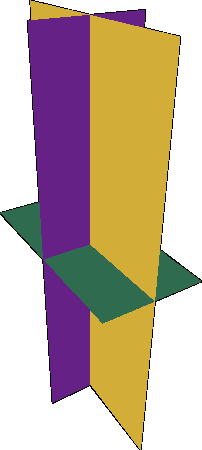
\includegraphics{asy/axesgraphic.pdf}}
  \put(9.5,-8.5){
\includegraphics{asy/shadow.pdf}}
  \put(15.25,-3){\makebox[0pt][r]{\frontcovertext{Linear Algebra}}}
  \put(15.25,-3.7){\makebox[0pt][r]{\frontcoverauthortext{Jim Hef{}feron}}}
  \put(15.25,-7.95){\makebox[0pt][r]{\frontcoverurltext{hefferon.net/linearalgebra}}}
  \put(15.25,-2.20){\makebox[0pt][r]{\frontcovereditiontext{Fourth edition}}}
  \put(7.65,-9.5){\spine}
  \put(1.0,-1.0){\backcoverhead}
  \put(1.0,-1.9){\backcovertext}

  \ifbool{showkdplinesbool}{% 
    % Front Cover width, height
    % Back cover
    \put(0.125,-0.125){\color{blue}\line(1,0){7.5}} % \FrontCoverWidth wide
      \put(0.125,-9.375){\color{blue}\line(1,0){7.5}} % \FrontCoverWidth wide
      \put(0.125,-0.125){\color{blue}\line(0,-1){9.25}} % \FrontCoverHeight tall
      \put(7.625,-0.125){\color{blue}\line(0,-1){9.25}}
    \put(0.25,-0.25){\color{blue}\line(1,0){7.375}} % \FrontCoverSafeWidth wide
      \put(0.25,-9.25){\color{blue}\line(1,0){7.375}} % \FrontCoverSafeWidth wide
      \put(0.25,-0.25){\color{blue}\line(0,-1){9.0}} % \FrontCoverSafeHeight tall
    % % Spine
    \put(7.687,-0.25){\color{blue}\line(1,0){1.071}} % 
      \put(7.687,-9.25){\color{blue}\line(1,0){1.071}} % 
    \put(7.687,-0.25){\color{blue}\line(0,-1){9}} %
      \put(8.758,-0.25){\color{blue}\line(0,-1){9}} %
    % % Front Cover
    \put(16.341,-0.125){\color{blue}\line(-1,0){7.5}} % 
      \put(16.341,-9.375){\color{blue}\line(-1,0){7.5}} % 
    \put(16.341,-0.125){\color{blue}\line(0,-1){9.25}} % 
      \put(8.821,-0.125){\color{blue}\line(0,-1){9.25}} % 
    \put(16.216,-0.25){\color{blue}\line(-1,0){7.375}} % Safe area
      \put(16.216,-9.25){\color{blue}\line(-1,0){7.375}} % 
    \put(16.216,-0.25){\color{blue}\line(0,-1){9}} % 
  }{}
\end{picture}
\end{document}
"
% See http://stackoverflow.com/a/1466610
\ifdefined\showguidelines
  \booltrue{showguidelinesbool}
\fi
\ifbool{showguidelinesbool}{\typeout{!!! GUIDELINES SHOWN}}{}
% Guidelines to show KDP lines.  Show or not?
\newbool{showkdplinesbool}
  % set the default by uncommenting one or the other
  \booltrue{showkdplinesbool} 
  % \boolfalse{showkdplinesbool}  
% You can cause KDP lines to be shown by invoking with
%   pdflatex "\def\showkdplines{}\documentclass{article}
% \usepackage{covergraphic}
\usepackage{graphicx}
\usepackage{ragged2e}
\usepackage{xcolor}
\colorlet{coverdarkcolor}{black}
\definecolor{coverbgcolor}{RGB}{212,175,55}  % gold
\definecolor{coverboldcolor}{RGB}{0,67,37}  % green
% \definecolor{coverboldcolor}{RGB}{103,0,153}  % purple

\usepackage[defaultsans]{lato}

\usepackage{stackengine}
\renewcommand{\stackalignment}{c}

% I want the booleans offered by this package
\usepackage{etoolbox}
% Guidelines help to arrange the parts visually.  Show or not?
\newbool{showguidelinesbool}
  % set the default by uncommenting one or the other
  % \booltrue{showguidelinesbool} 
  \boolfalse{showguidelinesbool}  
% You can cause guidelines to be shown by invoking with
%   pdflatex "\def\showguidelines{}\input{cover}"
% See http://stackoverflow.com/a/1466610
\ifdefined\showguidelines
  \booltrue{showguidelinesbool}
\fi
\ifbool{showguidelinesbool}{\typeout{!!! GUIDELINES SHOWN}}{}
% Guidelines to show KDP lines.  Show or not?
\newbool{showkdplinesbool}
  % set the default by uncommenting one or the other
  \booltrue{showkdplinesbool} 
  % \boolfalse{showkdplinesbool}  
% You can cause KDP lines to be shown by invoking with
%   pdflatex "\def\showkdplines{}\input{cover}"
\ifdefined\showkdplines
  \booltrue{showkdplinesbool}
\fi
\ifbool{showkdplinesbool}{\typeout{!!! KDP LINES SHOWN}}{}

% Size of page
% Kindle Direct Publishing gives this for a 531 page book;
% see the graphic KDP_diagram_531_pages.png
% # 	Description 	Width (in) 	Height (in)
% 1 	Full Cover 	16.446 	9.5
% 2 	Front Cover 	7.5 	9.25
% 3 	Safe Area 	7.375 	9
% 4 	Bleed 	0.125 	0.125
% 5 	Margin 	0.125 	0.125
% 6 	Spine 	1.196 	9.25
% 7 	Spine Safe Area 	1.071 	9
% 8 	Spine Margin 	0.062 	0.062
% 9 	Barcode Margin 	0.25 	0.25 

% I could calculate some of these from the others, but why?
% Number 3
\newlength{\FrontCoverSafeWidth}
  \setlength{\FrontCoverSafeWidth}{7.375in}
\newlength{\FrontCoverSafeHeight}
  \setlength{\FrontCoverSafeHeight}{9in}
% Number 5
\newlength{\FrontCoverMarginWidth}
  \setlength{\FrontCoverMarginWidth}{0.125in}
\newlength{\FrontCoverMarginHeight}
  \setlength{\FrontCoverMarginHeight}{0.125in}
% Number 2
\newlength{\FrontCoverWidth}
  \setlength{\FrontCoverWidth}{7.5in}
\newlength{\FrontCoverHeight}
  \setlength{\FrontCoverHeight}{9.25in}
% Number 4
\newlength{\BleedWidth}
  \setlength{\BleedWidth}{0.125in}
\newlength{\BleedHeight}
  \setlength{\BleedHeight}{0.125in}
% Number 7
\newlength{\SpineSafeWidth}
  \setlength{\SpineSafeWidth}{1.071in}
\newlength{\SpineSafeHeight}
  \setlength{\SpineSafeHeight}{9.0in}
% Number 8
\newlength{\SpineMarginWidth}
  \setlength{\SpineMarginWidth}{0.062in}
\newlength{\SpineMarginHeight}
  \setlength{\SpineMarginHeight}{0.062in}
% Number 9
\newlength{\BarcodeMarginWidth}
  \setlength{\BarcodeMarginWidth}{0.25in}
\newlength{\BarcodeMarginHeight}
  \setlength{\BarcodeMarginHeight}{0.25in}
% Number 6
\newlength{\SpineWidth}
  \setlength{\SpineWidth}{7.375in}
\newlength{\SpineHeight}
  \setlength{\SpineHeight}{9in}
% Number 1
\newlength{\FullCoverWidth}
  \setlength{\FullCoverWidth}{16.446in}
\newlength{\FullCoverHeight}
  \setlength{\FullCoverHeight}{9.5in}

\newlength{\totalcoverwidth} \setlength{\totalcoverwidth}{15.0in} % 7.5+7.5
\newlength{\spinewidth} \setlength{\spinewidth}{1in}
\addtolength{\totalcoverwidth}{\spinewidth}
\usepackage[papersize={16.446in,10in},margin=0in]{geometry}  

% ==== Spine ========
% 
\newcommand{\spinetext}[1]{\color{black}\fontsize{38pt}{8pt}{\fontfamily{ugq}\selectfont #1}}
\newcommand{\spineauthortext}[1]{\color{coverdarkcolor}\fontsize{23pt}{8pt}{\fontfamily{ugq}\selectfont{#1}}}
\newcommand{\spine}{%
\setlength{\unitlength}{1in}
\begin{picture}(1,9.5)
  \setstackgap{S}{2.1ex}
  % \put(0.235,5.65){\Shortstack{{\spinetext{L}} {\spinetext{I}} {\spinetext{N}} {\spinetext{E}} {\spinetext{A}} {\spinetext{R}}}}
  \put(0.18,8.5){\rotatebox[origin=lc]{-90}{\spinetext{Linear Algebra}\hspace{2.15in}\spineauthortext{Hef{}feron}}}
  \setstackgap{S}{0.9ex}
  % \put(0.3925,1.15){\Shortstack{{\spineauthortext{H}{14}} {\spineauthortext{E}{14}} {\spineauthortext{F}{14}} {\spineauthortext{F}{14}} {\spineauthortext{E}{14}} {\spineauthortext{R}{14}} {\spineauthortext{O}{14}} {\spineauthortext{N}{14}}}} % tried fake small caps by making the H be 14 pt, others be 11
\end{picture}
}


% ==== Back cover ========
% 
\newcommand{\backcovertext}{%
\RaggedRight
\color{black}\fontsize{14pt}{17pt}\fontfamily{fos}\selectfont
\begin{minipage}[t]{5.75in}
\setlength{\parskip}{1.4ex}
This text covers a standard first course:
Gauss's Method, vector spaces, linear maps and matrices, determinants,
and eigenvalues and eigenvectors.
In addition, each chapter ends with some
brief topics, including applications.

What sets this book apart is careful motivation, 
many examples, and extensive exercise sets.
Together, these help each student master the material of
the course and also help an instructor develop their student's  
level of mathematical maturity.

This book
has been freely available online for many years. 
It is widely used, 
both in classrooms and for self-study.
It is supported by worked answers for all exercises, 
projection slides for classroom use, 
and a lab manual based on \textit{Sage}. 

\vspace{.2in}
\noindent\textbf{Winner of the Math Association of America's Solow Award:}\\[1.35ex]
\vspace{-.225in}
\begin{center}
\parbox{5.5in}{
``The clear writing style, tremendous variety of exercises,
amenability to use with active learning strategies, and the
careful attention to detail in preparation mean that the text
is exceptionally adaptable.''}
\end{center}
\end{minipage}
}

\newcommand{\backcoverhead}{%
\setlength{\unitlength}{1in}
\begin{picture}(0,0)
  % \put(1,-.1){{\color{coverbgcolor}\rule{4.4in}{2pt}}}
  \put(0,-.1){{\color{coverbgcolor}\rule{5.05in}{2pt}}}
  \put(0.0,0){\color{coverboldcolor}\fontsize{25pt}{8pt}\fontfamily{fos}\selectfont \textit{A developmental approach to}}
  \put(3.0,-.45){\color{black}\fontsize{25pt}{8pt}\fontfamily{fos}\selectfont \textbf{Linear Algebra}}
\end{picture}
}




% ==== Front cover ========
% 
\newcommand{\frontcovertext}[1]{\color{black}\fontsize{55pt}{8pt}{\fontfamily{ugq}\selectfont #1}}
% \newcommand{\frontcovereditiontext}[1]{\color{black}\fontsize{20pt}{8pt}{\fontfamily{ugq}\selectfont #1}}
\newcommand{\frontcovereditiontext}[1]{\color[gray]{0.4}\fontsize{20pt}{6pt}\fontfamily{ugq}\selectfont \textsf{#1}}
% \newcommand{\frontcovereditiontext}[1]{\color{black}\fontsize{20pt}{6pt}\fontfamily{ugq}\selectfont #1}
\newcommand{\frontcoverauthortext}[1]{\color{black}\fontsize{27.5pt}{6pt}{\fontfamily{ugq}\selectfont #1}}
\newcommand{\frontcoverurltext}[1]{\color[gray]{0.4}\fontsize{18pt}{6pt}\fontfamily{ugq}\selectfont \textsf{#1}}
% \newcommand{\frontcoverurltext}[1]{\color[gray]{0.4}{\lato \fontsize{18pt}{6pt}\fontseries{sb}\selectfont #1}}


\setlength{\parindent}{0in}
\begin{document}\pagestyle{empty}\thispagestyle{empty}

\setlength{\unitlength}{1in}
\begin{picture}(0,0) 
  \ifbool{showguidelinesbool}{% 
    \put(0,-1){\makebox[0in]{\color{red}0}}
    \put(1,-1){\makebox[0in]{\color{red}1}}
    \put(2,-1){\makebox[0in]{\color{red}2}}
    \put(3,-1){\makebox[0in]{\color{red}3}}
    \put(4,-1){\makebox[0in]{\color{red}4}}
    \put(5,-1){\makebox[0in]{\color{red}5}}
    \put(6,-1){\makebox[0in]{\color{red}6}}
    \put(7,-1){\makebox[0in]{\color{red}7}}
    \put(7.5,-1){\color{red}\line(0,-1){8}}
    \put(8,-1){\makebox[0in]{\color{red}8}}
    \put(8,-1){\color{blue}\line(0,-1){8}}
    \put(8.5,-1){\color{red}\line(0,-1){8}}
    \put(9,-1){\makebox[0in]{\color{red}9}}
    \put(9.5,-1){\color{blue}\line(0,-1){8}}
    \put(10,-1){\makebox[0in]{\color{red}10}}
    \put(11,-1){\makebox[0in]{\color{red}11}}
    \put(12,-1){\makebox[0in]{\color{red}12}}
    \put(13,-1){\makebox[0in]{\color{red}13}}
    \put(14,-1){\makebox[0in]{\color{red}14}}
    \put(15,-1){\makebox[0in]{\color{red}15}}
    \put(15,-1){\color{blue}\line(0,-1){8}}
    \put(16,-1){\makebox[0in]{\color{red}16}}
  }{} 

  \put(9.5,-7.57){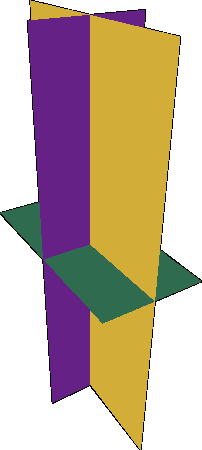
\includegraphics{asy/axesgraphic.pdf}}
  \put(9.5,-8.5){
\includegraphics{asy/shadow.pdf}}
  \put(15.25,-3){\makebox[0pt][r]{\frontcovertext{Linear Algebra}}}
  \put(15.25,-3.7){\makebox[0pt][r]{\frontcoverauthortext{Jim Hef{}feron}}}
  \put(15.25,-7.95){\makebox[0pt][r]{\frontcoverurltext{hefferon.net/linearalgebra}}}
  \put(15.25,-2.20){\makebox[0pt][r]{\frontcovereditiontext{Fourth edition}}}
  \put(7.65,-9.5){\spine}
  \put(1.0,-1.0){\backcoverhead}
  \put(1.0,-1.9){\backcovertext}

  \ifbool{showkdplinesbool}{% 
    % Front Cover width, height
    % Back cover
    \put(0.125,-0.125){\color{blue}\line(1,0){7.5}} % \FrontCoverWidth wide
      \put(0.125,-9.375){\color{blue}\line(1,0){7.5}} % \FrontCoverWidth wide
      \put(0.125,-0.125){\color{blue}\line(0,-1){9.25}} % \FrontCoverHeight tall
      \put(7.625,-0.125){\color{blue}\line(0,-1){9.25}}
    \put(0.25,-0.25){\color{blue}\line(1,0){7.375}} % \FrontCoverSafeWidth wide
      \put(0.25,-9.25){\color{blue}\line(1,0){7.375}} % \FrontCoverSafeWidth wide
      \put(0.25,-0.25){\color{blue}\line(0,-1){9.0}} % \FrontCoverSafeHeight tall
    % % Spine
    \put(7.687,-0.25){\color{blue}\line(1,0){1.071}} % 
      \put(7.687,-9.25){\color{blue}\line(1,0){1.071}} % 
    \put(7.687,-0.25){\color{blue}\line(0,-1){9}} %
      \put(8.758,-0.25){\color{blue}\line(0,-1){9}} %
    % % Front Cover
    \put(16.341,-0.125){\color{blue}\line(-1,0){7.5}} % 
      \put(16.341,-9.375){\color{blue}\line(-1,0){7.5}} % 
    \put(16.341,-0.125){\color{blue}\line(0,-1){9.25}} % 
      \put(8.821,-0.125){\color{blue}\line(0,-1){9.25}} % 
    \put(16.216,-0.25){\color{blue}\line(-1,0){7.375}} % Safe area
      \put(16.216,-9.25){\color{blue}\line(-1,0){7.375}} % 
    \put(16.216,-0.25){\color{blue}\line(0,-1){9}} % 
  }{}
\end{picture}
\end{document}
"
\ifdefined\showkdplines
  \booltrue{showkdplinesbool}
\fi
\ifbool{showkdplinesbool}{\typeout{!!! KDP LINES SHOWN}}{}

% Size of page
% Kindle Direct Publishing gives this for a 531 page book;
% see the graphic KDP_diagram_531_pages.png
% # 	Description 	Width (in) 	Height (in)
% 1 	Full Cover 	16.446 	9.5
% 2 	Front Cover 	7.5 	9.25
% 3 	Safe Area 	7.375 	9
% 4 	Bleed 	0.125 	0.125
% 5 	Margin 	0.125 	0.125
% 6 	Spine 	1.196 	9.25
% 7 	Spine Safe Area 	1.071 	9
% 8 	Spine Margin 	0.062 	0.062
% 9 	Barcode Margin 	0.25 	0.25 

% I could calculate some of these from the others, but why?
% Number 3
\newlength{\FrontCoverSafeWidth}
  \setlength{\FrontCoverSafeWidth}{7.375in}
\newlength{\FrontCoverSafeHeight}
  \setlength{\FrontCoverSafeHeight}{9in}
% Number 5
\newlength{\FrontCoverMarginWidth}
  \setlength{\FrontCoverMarginWidth}{0.125in}
\newlength{\FrontCoverMarginHeight}
  \setlength{\FrontCoverMarginHeight}{0.125in}
% Number 2
\newlength{\FrontCoverWidth}
  \setlength{\FrontCoverWidth}{7.5in}
\newlength{\FrontCoverHeight}
  \setlength{\FrontCoverHeight}{9.25in}
% Number 4
\newlength{\BleedWidth}
  \setlength{\BleedWidth}{0.125in}
\newlength{\BleedHeight}
  \setlength{\BleedHeight}{0.125in}
% Number 7
\newlength{\SpineSafeWidth}
  \setlength{\SpineSafeWidth}{1.071in}
\newlength{\SpineSafeHeight}
  \setlength{\SpineSafeHeight}{9.0in}
% Number 8
\newlength{\SpineMarginWidth}
  \setlength{\SpineMarginWidth}{0.062in}
\newlength{\SpineMarginHeight}
  \setlength{\SpineMarginHeight}{0.062in}
% Number 9
\newlength{\BarcodeMarginWidth}
  \setlength{\BarcodeMarginWidth}{0.25in}
\newlength{\BarcodeMarginHeight}
  \setlength{\BarcodeMarginHeight}{0.25in}
% Number 6
\newlength{\SpineWidth}
  \setlength{\SpineWidth}{7.375in}
\newlength{\SpineHeight}
  \setlength{\SpineHeight}{9in}
% Number 1
\newlength{\FullCoverWidth}
  \setlength{\FullCoverWidth}{16.446in}
\newlength{\FullCoverHeight}
  \setlength{\FullCoverHeight}{9.5in}

\newlength{\totalcoverwidth} \setlength{\totalcoverwidth}{15.0in} % 7.5+7.5
\newlength{\spinewidth} \setlength{\spinewidth}{1in}
\addtolength{\totalcoverwidth}{\spinewidth}
\usepackage[papersize={16.446in,10in},margin=0in]{geometry}  

% ==== Spine ========
% 
\newcommand{\spinetext}[1]{\color{black}\fontsize{38pt}{8pt}{\fontfamily{ugq}\selectfont #1}}
\newcommand{\spineauthortext}[1]{\color{coverdarkcolor}\fontsize{23pt}{8pt}{\fontfamily{ugq}\selectfont{#1}}}
\newcommand{\spine}{%
\setlength{\unitlength}{1in}
\begin{picture}(1,9.5)
  \setstackgap{S}{2.1ex}
  % \put(0.235,5.65){\Shortstack{{\spinetext{L}} {\spinetext{I}} {\spinetext{N}} {\spinetext{E}} {\spinetext{A}} {\spinetext{R}}}}
  \put(0.18,8.5){\rotatebox[origin=lc]{-90}{\spinetext{Linear Algebra}\hspace{2.15in}\spineauthortext{Hef{}feron}}}
  \setstackgap{S}{0.9ex}
  % \put(0.3925,1.15){\Shortstack{{\spineauthortext{H}{14}} {\spineauthortext{E}{14}} {\spineauthortext{F}{14}} {\spineauthortext{F}{14}} {\spineauthortext{E}{14}} {\spineauthortext{R}{14}} {\spineauthortext{O}{14}} {\spineauthortext{N}{14}}}} % tried fake small caps by making the H be 14 pt, others be 11
\end{picture}
}


% ==== Back cover ========
% 
\newcommand{\backcovertext}{%
\RaggedRight
\color{black}\fontsize{14pt}{17pt}\fontfamily{fos}\selectfont
\begin{minipage}[t]{5.75in}
\setlength{\parskip}{1.4ex}
This text covers a standard first course:
Gauss's Method, vector spaces, linear maps and matrices, determinants,
and eigenvalues and eigenvectors.
In addition, each chapter ends with some
brief topics, including applications.

What sets this book apart is careful motivation, 
many examples, and extensive exercise sets.
Together, these help each student master the material of
the course and also help an instructor develop their student's  
level of mathematical maturity.

This book
has been freely available online for many years. 
It is widely used, 
both in classrooms and for self-study.
It is supported by worked answers for all exercises, 
projection slides for classroom use, 
and a lab manual based on \textit{Sage}. 

\vspace{.2in}
\noindent\textbf{Winner of the Math Association of America's Solow Award:}\\[1.35ex]
\vspace{-.225in}
\begin{center}
\parbox{5.5in}{
``The clear writing style, tremendous variety of exercises,
amenability to use with active learning strategies, and the
careful attention to detail in preparation mean that the text
is exceptionally adaptable.''}
\end{center}
\end{minipage}
}

\newcommand{\backcoverhead}{%
\setlength{\unitlength}{1in}
\begin{picture}(0,0)
  % \put(1,-.1){{\color{coverbgcolor}\rule{4.4in}{2pt}}}
  \put(0,-.1){{\color{coverbgcolor}\rule{5.05in}{2pt}}}
  \put(0.0,0){\color{coverboldcolor}\fontsize{25pt}{8pt}\fontfamily{fos}\selectfont \textit{A developmental approach to}}
  \put(3.0,-.45){\color{black}\fontsize{25pt}{8pt}\fontfamily{fos}\selectfont \textbf{Linear Algebra}}
\end{picture}
}




% ==== Front cover ========
% 
\newcommand{\frontcovertext}[1]{\color{black}\fontsize{55pt}{8pt}{\fontfamily{ugq}\selectfont #1}}
% \newcommand{\frontcovereditiontext}[1]{\color{black}\fontsize{20pt}{8pt}{\fontfamily{ugq}\selectfont #1}}
\newcommand{\frontcovereditiontext}[1]{\color[gray]{0.4}\fontsize{20pt}{6pt}\fontfamily{ugq}\selectfont \textsf{#1}}
% \newcommand{\frontcovereditiontext}[1]{\color{black}\fontsize{20pt}{6pt}\fontfamily{ugq}\selectfont #1}
\newcommand{\frontcoverauthortext}[1]{\color{black}\fontsize{27.5pt}{6pt}{\fontfamily{ugq}\selectfont #1}}
\newcommand{\frontcoverurltext}[1]{\color[gray]{0.4}\fontsize{18pt}{6pt}\fontfamily{ugq}\selectfont \textsf{#1}}
% \newcommand{\frontcoverurltext}[1]{\color[gray]{0.4}{\lato \fontsize{18pt}{6pt}\fontseries{sb}\selectfont #1}}


\setlength{\parindent}{0in}
\begin{document}\pagestyle{empty}\thispagestyle{empty}

\setlength{\unitlength}{1in}
\begin{picture}(0,0) 
  \ifbool{showguidelinesbool}{% 
    \put(0,-1){\makebox[0in]{\color{red}0}}
    \put(1,-1){\makebox[0in]{\color{red}1}}
    \put(2,-1){\makebox[0in]{\color{red}2}}
    \put(3,-1){\makebox[0in]{\color{red}3}}
    \put(4,-1){\makebox[0in]{\color{red}4}}
    \put(5,-1){\makebox[0in]{\color{red}5}}
    \put(6,-1){\makebox[0in]{\color{red}6}}
    \put(7,-1){\makebox[0in]{\color{red}7}}
    \put(7.5,-1){\color{red}\line(0,-1){8}}
    \put(8,-1){\makebox[0in]{\color{red}8}}
    \put(8,-1){\color{blue}\line(0,-1){8}}
    \put(8.5,-1){\color{red}\line(0,-1){8}}
    \put(9,-1){\makebox[0in]{\color{red}9}}
    \put(9.5,-1){\color{blue}\line(0,-1){8}}
    \put(10,-1){\makebox[0in]{\color{red}10}}
    \put(11,-1){\makebox[0in]{\color{red}11}}
    \put(12,-1){\makebox[0in]{\color{red}12}}
    \put(13,-1){\makebox[0in]{\color{red}13}}
    \put(14,-1){\makebox[0in]{\color{red}14}}
    \put(15,-1){\makebox[0in]{\color{red}15}}
    \put(15,-1){\color{blue}\line(0,-1){8}}
    \put(16,-1){\makebox[0in]{\color{red}16}}
  }{} 

  \put(9.5,-7.57){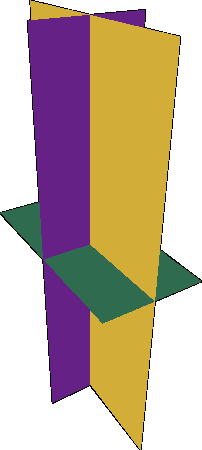
\includegraphics{asy/axesgraphic.pdf}}
  \put(9.5,-8.5){
\includegraphics{asy/shadow.pdf}}
  \put(15.25,-3){\makebox[0pt][r]{\frontcovertext{Linear Algebra}}}
  \put(15.25,-3.7){\makebox[0pt][r]{\frontcoverauthortext{Jim Hef{}feron}}}
  \put(15.25,-7.95){\makebox[0pt][r]{\frontcoverurltext{hefferon.net/linearalgebra}}}
  \put(15.25,-2.20){\makebox[0pt][r]{\frontcovereditiontext{Fourth edition}}}
  \put(7.65,-9.5){\spine}
  \put(1.0,-1.0){\backcoverhead}
  \put(1.0,-1.9){\backcovertext}

  \ifbool{showkdplinesbool}{% 
    % Front Cover width, height
    % Back cover
    \put(0.125,-0.125){\color{blue}\line(1,0){7.5}} % \FrontCoverWidth wide
      \put(0.125,-9.375){\color{blue}\line(1,0){7.5}} % \FrontCoverWidth wide
      \put(0.125,-0.125){\color{blue}\line(0,-1){9.25}} % \FrontCoverHeight tall
      \put(7.625,-0.125){\color{blue}\line(0,-1){9.25}}
    \put(0.25,-0.25){\color{blue}\line(1,0){7.375}} % \FrontCoverSafeWidth wide
      \put(0.25,-9.25){\color{blue}\line(1,0){7.375}} % \FrontCoverSafeWidth wide
      \put(0.25,-0.25){\color{blue}\line(0,-1){9.0}} % \FrontCoverSafeHeight tall
    % % Spine
    \put(7.687,-0.25){\color{blue}\line(1,0){1.071}} % 
      \put(7.687,-9.25){\color{blue}\line(1,0){1.071}} % 
    \put(7.687,-0.25){\color{blue}\line(0,-1){9}} %
      \put(8.758,-0.25){\color{blue}\line(0,-1){9}} %
    % % Front Cover
    \put(16.341,-0.125){\color{blue}\line(-1,0){7.5}} % 
      \put(16.341,-9.375){\color{blue}\line(-1,0){7.5}} % 
    \put(16.341,-0.125){\color{blue}\line(0,-1){9.25}} % 
      \put(8.821,-0.125){\color{blue}\line(0,-1){9.25}} % 
    \put(16.216,-0.25){\color{blue}\line(-1,0){7.375}} % Safe area
      \put(16.216,-9.25){\color{blue}\line(-1,0){7.375}} % 
    \put(16.216,-0.25){\color{blue}\line(0,-1){9}} % 
  }{}
\end{picture}
\end{document}
"
\ifdefined\showkdplines
  \booltrue{showkdplinesbool}
\fi
\ifbool{showkdplinesbool}{\typeout{!!! KDP LINES SHOWN}}{}

% Size of page
% Kindle Direct Publishing gives this for a 531 page book;
% see the graphic KDP_diagram_531_pages.png
% # 	Description 	Width (in) 	Height (in)
% 1 	Full Cover 	16.446 	9.5
% 2 	Front Cover 	7.5 	9.25
% 3 	Safe Area 	7.375 	9
% 4 	Bleed 	0.125 	0.125
% 5 	Margin 	0.125 	0.125
% 6 	Spine 	1.196 	9.25
% 7 	Spine Safe Area 	1.071 	9
% 8 	Spine Margin 	0.062 	0.062
% 9 	Barcode Margin 	0.25 	0.25 

% I could calculate some of these from the others, but why?
% Number 3
\newlength{\FrontCoverSafeWidth}
  \setlength{\FrontCoverSafeWidth}{7.375in}
\newlength{\FrontCoverSafeHeight}
  \setlength{\FrontCoverSafeHeight}{9in}
% Number 5
\newlength{\FrontCoverMarginWidth}
  \setlength{\FrontCoverMarginWidth}{0.125in}
\newlength{\FrontCoverMarginHeight}
  \setlength{\FrontCoverMarginHeight}{0.125in}
% Number 2
\newlength{\FrontCoverWidth}
  \setlength{\FrontCoverWidth}{7.5in}
\newlength{\FrontCoverHeight}
  \setlength{\FrontCoverHeight}{9.25in}
% Number 4
\newlength{\BleedWidth}
  \setlength{\BleedWidth}{0.125in}
\newlength{\BleedHeight}
  \setlength{\BleedHeight}{0.125in}
% Number 7
\newlength{\SpineSafeWidth}
  \setlength{\SpineSafeWidth}{1.071in}
\newlength{\SpineSafeHeight}
  \setlength{\SpineSafeHeight}{9.0in}
% Number 8
\newlength{\SpineMarginWidth}
  \setlength{\SpineMarginWidth}{0.062in}
\newlength{\SpineMarginHeight}
  \setlength{\SpineMarginHeight}{0.062in}
% Number 9
\newlength{\BarcodeMarginWidth}
  \setlength{\BarcodeMarginWidth}{0.25in}
\newlength{\BarcodeMarginHeight}
  \setlength{\BarcodeMarginHeight}{0.25in}
% Number 6
\newlength{\SpineWidth}
  \setlength{\SpineWidth}{7.375in}
\newlength{\SpineHeight}
  \setlength{\SpineHeight}{9in}
% Number 1
\newlength{\FullCoverWidth}
  \setlength{\FullCoverWidth}{16.446in}
\newlength{\FullCoverHeight}
  \setlength{\FullCoverHeight}{9.5in}

\newlength{\totalcoverwidth} \setlength{\totalcoverwidth}{15.0in} % 7.5+7.5
\newlength{\spinewidth} \setlength{\spinewidth}{1in}
\addtolength{\totalcoverwidth}{\spinewidth}
\usepackage[papersize={16.446in,10in},margin=0in]{geometry}  

% ==== Spine ========
% 
\newcommand{\spinetext}[1]{\color{black}\fontsize{38pt}{8pt}{\fontfamily{ugq}\selectfont #1}}
\newcommand{\spineauthortext}[1]{\color{coverdarkcolor}\fontsize{23pt}{8pt}{\fontfamily{ugq}\selectfont{#1}}}
\newcommand{\spine}{%
\setlength{\unitlength}{1in}
\begin{picture}(1,9.5)
  \setstackgap{S}{2.1ex}
  % \put(0.235,5.65){\Shortstack{{\spinetext{L}} {\spinetext{I}} {\spinetext{N}} {\spinetext{E}} {\spinetext{A}} {\spinetext{R}}}}
  \put(0.18,8.5){\rotatebox[origin=lc]{-90}{\spinetext{Linear Algebra}\hspace{2.15in}\spineauthortext{Hef{}feron}}}
  \setstackgap{S}{0.9ex}
  % \put(0.3925,1.15){\Shortstack{{\spineauthortext{H}{14}} {\spineauthortext{E}{14}} {\spineauthortext{F}{14}} {\spineauthortext{F}{14}} {\spineauthortext{E}{14}} {\spineauthortext{R}{14}} {\spineauthortext{O}{14}} {\spineauthortext{N}{14}}}} % tried fake small caps by making the H be 14 pt, others be 11
\end{picture}
}


% ==== Back cover ========
% 
\newcommand{\backcovertext}{%
\RaggedRight
\color{black}\fontsize{14pt}{17pt}\fontfamily{fos}\selectfont
\begin{minipage}[t]{5.75in}
\setlength{\parskip}{1.4ex}
This text covers a standard first course:
Gauss's Method, vector spaces, linear maps and matrices, determinants,
and eigenvalues and eigenvectors.
In addition, each chapter ends with some
brief topics, including applications.

What sets this book apart is careful motivation, 
many examples, and extensive exercise sets.
Together, these help each student master the material of
the course and also help an instructor develop their student's  
level of mathematical maturity.

This book
has been freely available online for many years. 
It is widely used, 
both in classrooms and for self-study.
It is supported by worked answers for all exercises, 
projection slides for classroom use, 
and a lab manual based on \textit{Sage}. 

\vspace{.2in}
\noindent\textbf{Winner of the Math Association of America's Solow Award:}\\[1.35ex]
\vspace{-.225in}
\begin{center}
\parbox{5.5in}{
``The clear writing style, tremendous variety of exercises,
amenability to use with active learning strategies, and the
careful attention to detail in preparation mean that the text
is exceptionally adaptable.''}
\end{center}
\end{minipage}
}

\newcommand{\backcoverhead}{%
\setlength{\unitlength}{1in}
\begin{picture}(0,0)
  % \put(1,-.1){{\color{coverbgcolor}\rule{4.4in}{2pt}}}
  \put(0,-.1){{\color{coverbgcolor}\rule{5.05in}{2pt}}}
  \put(0.0,0){\color{coverboldcolor}\fontsize{25pt}{8pt}\fontfamily{fos}\selectfont \textit{A developmental approach to}}
  \put(3.0,-.45){\color{black}\fontsize{25pt}{8pt}\fontfamily{fos}\selectfont \textbf{Linear Algebra}}
\end{picture}
}




% ==== Front cover ========
% 
\newcommand{\frontcovertext}[1]{\color{black}\fontsize{55pt}{8pt}{\fontfamily{ugq}\selectfont #1}}
% \newcommand{\frontcovereditiontext}[1]{\color{black}\fontsize{20pt}{8pt}{\fontfamily{ugq}\selectfont #1}}
\newcommand{\frontcovereditiontext}[1]{\color[gray]{0.4}\fontsize{20pt}{6pt}\fontfamily{ugq}\selectfont \textsf{#1}}
% \newcommand{\frontcovereditiontext}[1]{\color{black}\fontsize{20pt}{6pt}\fontfamily{ugq}\selectfont #1}
\newcommand{\frontcoverauthortext}[1]{\color{black}\fontsize{27.5pt}{6pt}{\fontfamily{ugq}\selectfont #1}}
\newcommand{\frontcoverurltext}[1]{\color[gray]{0.4}\fontsize{18pt}{6pt}\fontfamily{ugq}\selectfont \textsf{#1}}
% \newcommand{\frontcoverurltext}[1]{\color[gray]{0.4}{\lato \fontsize{18pt}{6pt}\fontseries{sb}\selectfont #1}}


\setlength{\parindent}{0in}
\begin{document}\pagestyle{empty}\thispagestyle{empty}

\setlength{\unitlength}{1in}
\begin{picture}(0,0) 
  \ifbool{showguidelinesbool}{% 
    \put(0,-1){\makebox[0in]{\color{red}0}}
    \put(1,-1){\makebox[0in]{\color{red}1}}
    \put(2,-1){\makebox[0in]{\color{red}2}}
    \put(3,-1){\makebox[0in]{\color{red}3}}
    \put(4,-1){\makebox[0in]{\color{red}4}}
    \put(5,-1){\makebox[0in]{\color{red}5}}
    \put(6,-1){\makebox[0in]{\color{red}6}}
    \put(7,-1){\makebox[0in]{\color{red}7}}
    \put(7.5,-1){\color{red}\line(0,-1){8}}
    \put(8,-1){\makebox[0in]{\color{red}8}}
    \put(8,-1){\color{blue}\line(0,-1){8}}
    \put(8.5,-1){\color{red}\line(0,-1){8}}
    \put(9,-1){\makebox[0in]{\color{red}9}}
    \put(9.5,-1){\color{blue}\line(0,-1){8}}
    \put(10,-1){\makebox[0in]{\color{red}10}}
    \put(11,-1){\makebox[0in]{\color{red}11}}
    \put(12,-1){\makebox[0in]{\color{red}12}}
    \put(13,-1){\makebox[0in]{\color{red}13}}
    \put(14,-1){\makebox[0in]{\color{red}14}}
    \put(15,-1){\makebox[0in]{\color{red}15}}
    \put(15,-1){\color{blue}\line(0,-1){8}}
    \put(16,-1){\makebox[0in]{\color{red}16}}
  }{} 

  \put(9.5,-7.57){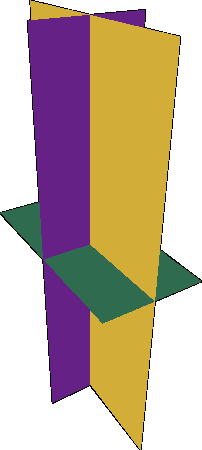
\includegraphics{asy/axesgraphic.pdf}}
  \put(9.5,-8.5){
\includegraphics{asy/shadow.pdf}}
  \put(15.25,-3){\makebox[0pt][r]{\frontcovertext{Linear Algebra}}}
  \put(15.25,-3.7){\makebox[0pt][r]{\frontcoverauthortext{Jim Hef{}feron}}}
  \put(15.25,-7.95){\makebox[0pt][r]{\frontcoverurltext{hefferon.net/linearalgebra}}}
  \put(15.25,-2.20){\makebox[0pt][r]{\frontcovereditiontext{Fourth edition}}}
  \put(7.65,-9.5){\spine}
  \put(1.0,-1.0){\backcoverhead}
  \put(1.0,-1.9){\backcovertext}

  \ifbool{showkdplinesbool}{% 
    % Front Cover width, height
    % Back cover
    \put(0.125,-0.125){\color{blue}\line(1,0){7.5}} % \FrontCoverWidth wide
      \put(0.125,-9.375){\color{blue}\line(1,0){7.5}} % \FrontCoverWidth wide
      \put(0.125,-0.125){\color{blue}\line(0,-1){9.25}} % \FrontCoverHeight tall
      \put(7.625,-0.125){\color{blue}\line(0,-1){9.25}}
    \put(0.25,-0.25){\color{blue}\line(1,0){7.375}} % \FrontCoverSafeWidth wide
      \put(0.25,-9.25){\color{blue}\line(1,0){7.375}} % \FrontCoverSafeWidth wide
      \put(0.25,-0.25){\color{blue}\line(0,-1){9.0}} % \FrontCoverSafeHeight tall
    % % Spine
    \put(7.687,-0.25){\color{blue}\line(1,0){1.071}} % 
      \put(7.687,-9.25){\color{blue}\line(1,0){1.071}} % 
    \put(7.687,-0.25){\color{blue}\line(0,-1){9}} %
      \put(8.758,-0.25){\color{blue}\line(0,-1){9}} %
    % % Front Cover
    \put(16.341,-0.125){\color{blue}\line(-1,0){7.5}} % 
      \put(16.341,-9.375){\color{blue}\line(-1,0){7.5}} % 
    \put(16.341,-0.125){\color{blue}\line(0,-1){9.25}} % 
      \put(8.821,-0.125){\color{blue}\line(0,-1){9.25}} % 
    \put(16.216,-0.25){\color{blue}\line(-1,0){7.375}} % Safe area
      \put(16.216,-9.25){\color{blue}\line(-1,0){7.375}} % 
    \put(16.216,-0.25){\color{blue}\line(0,-1){9}} % 
  }{}
\end{picture}
\end{document}
"
% See http://stackoverflow.com/a/1466610
\ifdefined\showguidelines
  \booltrue{showguidelinesbool}
\fi
\ifbool{showguidelinesbool}{\typeout{!!! GUIDELINES SHOWN}}{}
% Guidelines to show KDP lines.  Show or not?
\newbool{showkdplinesbool}
  % set the default by uncommenting one or the other
  \booltrue{showkdplinesbool} 
  % \boolfalse{showkdplinesbool}  
% You can cause KDP lines to be shown by invoking with
%   pdflatex "\def\showkdplines{}\documentclass{article}
% \usepackage{covergraphic}
\usepackage{graphicx}
\usepackage{ragged2e}
\usepackage{xcolor}
\colorlet{coverdarkcolor}{black}
\definecolor{coverbgcolor}{RGB}{212,175,55}  % gold
\definecolor{coverboldcolor}{RGB}{0,67,37}  % green
% \definecolor{coverboldcolor}{RGB}{103,0,153}  % purple

\usepackage[defaultsans]{lato}

\usepackage{stackengine}
\renewcommand{\stackalignment}{c}

% I want the booleans offered by this package
\usepackage{etoolbox}
% Guidelines help to arrange the parts visually.  Show or not?
\newbool{showguidelinesbool}
  % set the default by uncommenting one or the other
  % \booltrue{showguidelinesbool} 
  \boolfalse{showguidelinesbool}  
% You can cause guidelines to be shown by invoking with
%   pdflatex "\def\showguidelines{}\documentclass{article}
% \usepackage{covergraphic}
\usepackage{graphicx}
\usepackage{ragged2e}
\usepackage{xcolor}
\colorlet{coverdarkcolor}{black}
\definecolor{coverbgcolor}{RGB}{212,175,55}  % gold
\definecolor{coverboldcolor}{RGB}{0,67,37}  % green
% \definecolor{coverboldcolor}{RGB}{103,0,153}  % purple

\usepackage[defaultsans]{lato}

\usepackage{stackengine}
\renewcommand{\stackalignment}{c}

% I want the booleans offered by this package
\usepackage{etoolbox}
% Guidelines help to arrange the parts visually.  Show or not?
\newbool{showguidelinesbool}
  % set the default by uncommenting one or the other
  % \booltrue{showguidelinesbool} 
  \boolfalse{showguidelinesbool}  
% You can cause guidelines to be shown by invoking with
%   pdflatex "\def\showguidelines{}\documentclass{article}
% \usepackage{covergraphic}
\usepackage{graphicx}
\usepackage{ragged2e}
\usepackage{xcolor}
\colorlet{coverdarkcolor}{black}
\definecolor{coverbgcolor}{RGB}{212,175,55}  % gold
\definecolor{coverboldcolor}{RGB}{0,67,37}  % green
% \definecolor{coverboldcolor}{RGB}{103,0,153}  % purple

\usepackage[defaultsans]{lato}

\usepackage{stackengine}
\renewcommand{\stackalignment}{c}

% I want the booleans offered by this package
\usepackage{etoolbox}
% Guidelines help to arrange the parts visually.  Show or not?
\newbool{showguidelinesbool}
  % set the default by uncommenting one or the other
  % \booltrue{showguidelinesbool} 
  \boolfalse{showguidelinesbool}  
% You can cause guidelines to be shown by invoking with
%   pdflatex "\def\showguidelines{}\input{cover}"
% See http://stackoverflow.com/a/1466610
\ifdefined\showguidelines
  \booltrue{showguidelinesbool}
\fi
\ifbool{showguidelinesbool}{\typeout{!!! GUIDELINES SHOWN}}{}
% Guidelines to show KDP lines.  Show or not?
\newbool{showkdplinesbool}
  % set the default by uncommenting one or the other
  \booltrue{showkdplinesbool} 
  % \boolfalse{showkdplinesbool}  
% You can cause KDP lines to be shown by invoking with
%   pdflatex "\def\showkdplines{}\input{cover}"
\ifdefined\showkdplines
  \booltrue{showkdplinesbool}
\fi
\ifbool{showkdplinesbool}{\typeout{!!! KDP LINES SHOWN}}{}

% Size of page
% Kindle Direct Publishing gives this for a 531 page book;
% see the graphic KDP_diagram_531_pages.png
% # 	Description 	Width (in) 	Height (in)
% 1 	Full Cover 	16.446 	9.5
% 2 	Front Cover 	7.5 	9.25
% 3 	Safe Area 	7.375 	9
% 4 	Bleed 	0.125 	0.125
% 5 	Margin 	0.125 	0.125
% 6 	Spine 	1.196 	9.25
% 7 	Spine Safe Area 	1.071 	9
% 8 	Spine Margin 	0.062 	0.062
% 9 	Barcode Margin 	0.25 	0.25 

% I could calculate some of these from the others, but why?
% Number 3
\newlength{\FrontCoverSafeWidth}
  \setlength{\FrontCoverSafeWidth}{7.375in}
\newlength{\FrontCoverSafeHeight}
  \setlength{\FrontCoverSafeHeight}{9in}
% Number 5
\newlength{\FrontCoverMarginWidth}
  \setlength{\FrontCoverMarginWidth}{0.125in}
\newlength{\FrontCoverMarginHeight}
  \setlength{\FrontCoverMarginHeight}{0.125in}
% Number 2
\newlength{\FrontCoverWidth}
  \setlength{\FrontCoverWidth}{7.5in}
\newlength{\FrontCoverHeight}
  \setlength{\FrontCoverHeight}{9.25in}
% Number 4
\newlength{\BleedWidth}
  \setlength{\BleedWidth}{0.125in}
\newlength{\BleedHeight}
  \setlength{\BleedHeight}{0.125in}
% Number 7
\newlength{\SpineSafeWidth}
  \setlength{\SpineSafeWidth}{1.071in}
\newlength{\SpineSafeHeight}
  \setlength{\SpineSafeHeight}{9.0in}
% Number 8
\newlength{\SpineMarginWidth}
  \setlength{\SpineMarginWidth}{0.062in}
\newlength{\SpineMarginHeight}
  \setlength{\SpineMarginHeight}{0.062in}
% Number 9
\newlength{\BarcodeMarginWidth}
  \setlength{\BarcodeMarginWidth}{0.25in}
\newlength{\BarcodeMarginHeight}
  \setlength{\BarcodeMarginHeight}{0.25in}
% Number 6
\newlength{\SpineWidth}
  \setlength{\SpineWidth}{7.375in}
\newlength{\SpineHeight}
  \setlength{\SpineHeight}{9in}
% Number 1
\newlength{\FullCoverWidth}
  \setlength{\FullCoverWidth}{16.446in}
\newlength{\FullCoverHeight}
  \setlength{\FullCoverHeight}{9.5in}

\newlength{\totalcoverwidth} \setlength{\totalcoverwidth}{15.0in} % 7.5+7.5
\newlength{\spinewidth} \setlength{\spinewidth}{1in}
\addtolength{\totalcoverwidth}{\spinewidth}
\usepackage[papersize={16.446in,10in},margin=0in]{geometry}  

% ==== Spine ========
% 
\newcommand{\spinetext}[1]{\color{black}\fontsize{38pt}{8pt}{\fontfamily{ugq}\selectfont #1}}
\newcommand{\spineauthortext}[1]{\color{coverdarkcolor}\fontsize{23pt}{8pt}{\fontfamily{ugq}\selectfont{#1}}}
\newcommand{\spine}{%
\setlength{\unitlength}{1in}
\begin{picture}(1,9.5)
  \setstackgap{S}{2.1ex}
  % \put(0.235,5.65){\Shortstack{{\spinetext{L}} {\spinetext{I}} {\spinetext{N}} {\spinetext{E}} {\spinetext{A}} {\spinetext{R}}}}
  \put(0.18,8.5){\rotatebox[origin=lc]{-90}{\spinetext{Linear Algebra}\hspace{2.15in}\spineauthortext{Hef{}feron}}}
  \setstackgap{S}{0.9ex}
  % \put(0.3925,1.15){\Shortstack{{\spineauthortext{H}{14}} {\spineauthortext{E}{14}} {\spineauthortext{F}{14}} {\spineauthortext{F}{14}} {\spineauthortext{E}{14}} {\spineauthortext{R}{14}} {\spineauthortext{O}{14}} {\spineauthortext{N}{14}}}} % tried fake small caps by making the H be 14 pt, others be 11
\end{picture}
}


% ==== Back cover ========
% 
\newcommand{\backcovertext}{%
\RaggedRight
\color{black}\fontsize{14pt}{17pt}\fontfamily{fos}\selectfont
\begin{minipage}[t]{5.75in}
\setlength{\parskip}{1.4ex}
This text covers a standard first course:
Gauss's Method, vector spaces, linear maps and matrices, determinants,
and eigenvalues and eigenvectors.
In addition, each chapter ends with some
brief topics, including applications.

What sets this book apart is careful motivation, 
many examples, and extensive exercise sets.
Together, these help each student master the material of
the course and also help an instructor develop their student's  
level of mathematical maturity.

This book
has been freely available online for many years. 
It is widely used, 
both in classrooms and for self-study.
It is supported by worked answers for all exercises, 
projection slides for classroom use, 
and a lab manual based on \textit{Sage}. 

\vspace{.2in}
\noindent\textbf{Winner of the Math Association of America's Solow Award:}\\[1.35ex]
\vspace{-.225in}
\begin{center}
\parbox{5.5in}{
``The clear writing style, tremendous variety of exercises,
amenability to use with active learning strategies, and the
careful attention to detail in preparation mean that the text
is exceptionally adaptable.''}
\end{center}
\end{minipage}
}

\newcommand{\backcoverhead}{%
\setlength{\unitlength}{1in}
\begin{picture}(0,0)
  % \put(1,-.1){{\color{coverbgcolor}\rule{4.4in}{2pt}}}
  \put(0,-.1){{\color{coverbgcolor}\rule{5.05in}{2pt}}}
  \put(0.0,0){\color{coverboldcolor}\fontsize{25pt}{8pt}\fontfamily{fos}\selectfont \textit{A developmental approach to}}
  \put(3.0,-.45){\color{black}\fontsize{25pt}{8pt}\fontfamily{fos}\selectfont \textbf{Linear Algebra}}
\end{picture}
}




% ==== Front cover ========
% 
\newcommand{\frontcovertext}[1]{\color{black}\fontsize{55pt}{8pt}{\fontfamily{ugq}\selectfont #1}}
% \newcommand{\frontcovereditiontext}[1]{\color{black}\fontsize{20pt}{8pt}{\fontfamily{ugq}\selectfont #1}}
\newcommand{\frontcovereditiontext}[1]{\color[gray]{0.4}\fontsize{20pt}{6pt}\fontfamily{ugq}\selectfont \textsf{#1}}
% \newcommand{\frontcovereditiontext}[1]{\color{black}\fontsize{20pt}{6pt}\fontfamily{ugq}\selectfont #1}
\newcommand{\frontcoverauthortext}[1]{\color{black}\fontsize{27.5pt}{6pt}{\fontfamily{ugq}\selectfont #1}}
\newcommand{\frontcoverurltext}[1]{\color[gray]{0.4}\fontsize{18pt}{6pt}\fontfamily{ugq}\selectfont \textsf{#1}}
% \newcommand{\frontcoverurltext}[1]{\color[gray]{0.4}{\lato \fontsize{18pt}{6pt}\fontseries{sb}\selectfont #1}}


\setlength{\parindent}{0in}
\begin{document}\pagestyle{empty}\thispagestyle{empty}

\setlength{\unitlength}{1in}
\begin{picture}(0,0) 
  \ifbool{showguidelinesbool}{% 
    \put(0,-1){\makebox[0in]{\color{red}0}}
    \put(1,-1){\makebox[0in]{\color{red}1}}
    \put(2,-1){\makebox[0in]{\color{red}2}}
    \put(3,-1){\makebox[0in]{\color{red}3}}
    \put(4,-1){\makebox[0in]{\color{red}4}}
    \put(5,-1){\makebox[0in]{\color{red}5}}
    \put(6,-1){\makebox[0in]{\color{red}6}}
    \put(7,-1){\makebox[0in]{\color{red}7}}
    \put(7.5,-1){\color{red}\line(0,-1){8}}
    \put(8,-1){\makebox[0in]{\color{red}8}}
    \put(8,-1){\color{blue}\line(0,-1){8}}
    \put(8.5,-1){\color{red}\line(0,-1){8}}
    \put(9,-1){\makebox[0in]{\color{red}9}}
    \put(9.5,-1){\color{blue}\line(0,-1){8}}
    \put(10,-1){\makebox[0in]{\color{red}10}}
    \put(11,-1){\makebox[0in]{\color{red}11}}
    \put(12,-1){\makebox[0in]{\color{red}12}}
    \put(13,-1){\makebox[0in]{\color{red}13}}
    \put(14,-1){\makebox[0in]{\color{red}14}}
    \put(15,-1){\makebox[0in]{\color{red}15}}
    \put(15,-1){\color{blue}\line(0,-1){8}}
    \put(16,-1){\makebox[0in]{\color{red}16}}
  }{} 

  \put(9.5,-7.57){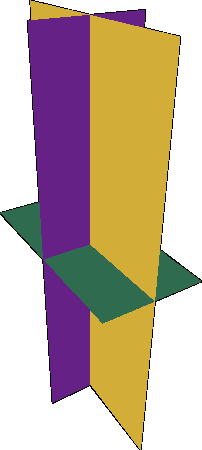
\includegraphics{asy/axesgraphic.pdf}}
  \put(9.5,-8.5){
\includegraphics{asy/shadow.pdf}}
  \put(15.25,-3){\makebox[0pt][r]{\frontcovertext{Linear Algebra}}}
  \put(15.25,-3.7){\makebox[0pt][r]{\frontcoverauthortext{Jim Hef{}feron}}}
  \put(15.25,-7.95){\makebox[0pt][r]{\frontcoverurltext{hefferon.net/linearalgebra}}}
  \put(15.25,-2.20){\makebox[0pt][r]{\frontcovereditiontext{Fourth edition}}}
  \put(7.65,-9.5){\spine}
  \put(1.0,-1.0){\backcoverhead}
  \put(1.0,-1.9){\backcovertext}

  \ifbool{showkdplinesbool}{% 
    % Front Cover width, height
    % Back cover
    \put(0.125,-0.125){\color{blue}\line(1,0){7.5}} % \FrontCoverWidth wide
      \put(0.125,-9.375){\color{blue}\line(1,0){7.5}} % \FrontCoverWidth wide
      \put(0.125,-0.125){\color{blue}\line(0,-1){9.25}} % \FrontCoverHeight tall
      \put(7.625,-0.125){\color{blue}\line(0,-1){9.25}}
    \put(0.25,-0.25){\color{blue}\line(1,0){7.375}} % \FrontCoverSafeWidth wide
      \put(0.25,-9.25){\color{blue}\line(1,0){7.375}} % \FrontCoverSafeWidth wide
      \put(0.25,-0.25){\color{blue}\line(0,-1){9.0}} % \FrontCoverSafeHeight tall
    % % Spine
    \put(7.687,-0.25){\color{blue}\line(1,0){1.071}} % 
      \put(7.687,-9.25){\color{blue}\line(1,0){1.071}} % 
    \put(7.687,-0.25){\color{blue}\line(0,-1){9}} %
      \put(8.758,-0.25){\color{blue}\line(0,-1){9}} %
    % % Front Cover
    \put(16.341,-0.125){\color{blue}\line(-1,0){7.5}} % 
      \put(16.341,-9.375){\color{blue}\line(-1,0){7.5}} % 
    \put(16.341,-0.125){\color{blue}\line(0,-1){9.25}} % 
      \put(8.821,-0.125){\color{blue}\line(0,-1){9.25}} % 
    \put(16.216,-0.25){\color{blue}\line(-1,0){7.375}} % Safe area
      \put(16.216,-9.25){\color{blue}\line(-1,0){7.375}} % 
    \put(16.216,-0.25){\color{blue}\line(0,-1){9}} % 
  }{}
\end{picture}
\end{document}
"
% See http://stackoverflow.com/a/1466610
\ifdefined\showguidelines
  \booltrue{showguidelinesbool}
\fi
\ifbool{showguidelinesbool}{\typeout{!!! GUIDELINES SHOWN}}{}
% Guidelines to show KDP lines.  Show or not?
\newbool{showkdplinesbool}
  % set the default by uncommenting one or the other
  \booltrue{showkdplinesbool} 
  % \boolfalse{showkdplinesbool}  
% You can cause KDP lines to be shown by invoking with
%   pdflatex "\def\showkdplines{}\documentclass{article}
% \usepackage{covergraphic}
\usepackage{graphicx}
\usepackage{ragged2e}
\usepackage{xcolor}
\colorlet{coverdarkcolor}{black}
\definecolor{coverbgcolor}{RGB}{212,175,55}  % gold
\definecolor{coverboldcolor}{RGB}{0,67,37}  % green
% \definecolor{coverboldcolor}{RGB}{103,0,153}  % purple

\usepackage[defaultsans]{lato}

\usepackage{stackengine}
\renewcommand{\stackalignment}{c}

% I want the booleans offered by this package
\usepackage{etoolbox}
% Guidelines help to arrange the parts visually.  Show or not?
\newbool{showguidelinesbool}
  % set the default by uncommenting one or the other
  % \booltrue{showguidelinesbool} 
  \boolfalse{showguidelinesbool}  
% You can cause guidelines to be shown by invoking with
%   pdflatex "\def\showguidelines{}\input{cover}"
% See http://stackoverflow.com/a/1466610
\ifdefined\showguidelines
  \booltrue{showguidelinesbool}
\fi
\ifbool{showguidelinesbool}{\typeout{!!! GUIDELINES SHOWN}}{}
% Guidelines to show KDP lines.  Show or not?
\newbool{showkdplinesbool}
  % set the default by uncommenting one or the other
  \booltrue{showkdplinesbool} 
  % \boolfalse{showkdplinesbool}  
% You can cause KDP lines to be shown by invoking with
%   pdflatex "\def\showkdplines{}\input{cover}"
\ifdefined\showkdplines
  \booltrue{showkdplinesbool}
\fi
\ifbool{showkdplinesbool}{\typeout{!!! KDP LINES SHOWN}}{}

% Size of page
% Kindle Direct Publishing gives this for a 531 page book;
% see the graphic KDP_diagram_531_pages.png
% # 	Description 	Width (in) 	Height (in)
% 1 	Full Cover 	16.446 	9.5
% 2 	Front Cover 	7.5 	9.25
% 3 	Safe Area 	7.375 	9
% 4 	Bleed 	0.125 	0.125
% 5 	Margin 	0.125 	0.125
% 6 	Spine 	1.196 	9.25
% 7 	Spine Safe Area 	1.071 	9
% 8 	Spine Margin 	0.062 	0.062
% 9 	Barcode Margin 	0.25 	0.25 

% I could calculate some of these from the others, but why?
% Number 3
\newlength{\FrontCoverSafeWidth}
  \setlength{\FrontCoverSafeWidth}{7.375in}
\newlength{\FrontCoverSafeHeight}
  \setlength{\FrontCoverSafeHeight}{9in}
% Number 5
\newlength{\FrontCoverMarginWidth}
  \setlength{\FrontCoverMarginWidth}{0.125in}
\newlength{\FrontCoverMarginHeight}
  \setlength{\FrontCoverMarginHeight}{0.125in}
% Number 2
\newlength{\FrontCoverWidth}
  \setlength{\FrontCoverWidth}{7.5in}
\newlength{\FrontCoverHeight}
  \setlength{\FrontCoverHeight}{9.25in}
% Number 4
\newlength{\BleedWidth}
  \setlength{\BleedWidth}{0.125in}
\newlength{\BleedHeight}
  \setlength{\BleedHeight}{0.125in}
% Number 7
\newlength{\SpineSafeWidth}
  \setlength{\SpineSafeWidth}{1.071in}
\newlength{\SpineSafeHeight}
  \setlength{\SpineSafeHeight}{9.0in}
% Number 8
\newlength{\SpineMarginWidth}
  \setlength{\SpineMarginWidth}{0.062in}
\newlength{\SpineMarginHeight}
  \setlength{\SpineMarginHeight}{0.062in}
% Number 9
\newlength{\BarcodeMarginWidth}
  \setlength{\BarcodeMarginWidth}{0.25in}
\newlength{\BarcodeMarginHeight}
  \setlength{\BarcodeMarginHeight}{0.25in}
% Number 6
\newlength{\SpineWidth}
  \setlength{\SpineWidth}{7.375in}
\newlength{\SpineHeight}
  \setlength{\SpineHeight}{9in}
% Number 1
\newlength{\FullCoverWidth}
  \setlength{\FullCoverWidth}{16.446in}
\newlength{\FullCoverHeight}
  \setlength{\FullCoverHeight}{9.5in}

\newlength{\totalcoverwidth} \setlength{\totalcoverwidth}{15.0in} % 7.5+7.5
\newlength{\spinewidth} \setlength{\spinewidth}{1in}
\addtolength{\totalcoverwidth}{\spinewidth}
\usepackage[papersize={16.446in,10in},margin=0in]{geometry}  

% ==== Spine ========
% 
\newcommand{\spinetext}[1]{\color{black}\fontsize{38pt}{8pt}{\fontfamily{ugq}\selectfont #1}}
\newcommand{\spineauthortext}[1]{\color{coverdarkcolor}\fontsize{23pt}{8pt}{\fontfamily{ugq}\selectfont{#1}}}
\newcommand{\spine}{%
\setlength{\unitlength}{1in}
\begin{picture}(1,9.5)
  \setstackgap{S}{2.1ex}
  % \put(0.235,5.65){\Shortstack{{\spinetext{L}} {\spinetext{I}} {\spinetext{N}} {\spinetext{E}} {\spinetext{A}} {\spinetext{R}}}}
  \put(0.18,8.5){\rotatebox[origin=lc]{-90}{\spinetext{Linear Algebra}\hspace{2.15in}\spineauthortext{Hef{}feron}}}
  \setstackgap{S}{0.9ex}
  % \put(0.3925,1.15){\Shortstack{{\spineauthortext{H}{14}} {\spineauthortext{E}{14}} {\spineauthortext{F}{14}} {\spineauthortext{F}{14}} {\spineauthortext{E}{14}} {\spineauthortext{R}{14}} {\spineauthortext{O}{14}} {\spineauthortext{N}{14}}}} % tried fake small caps by making the H be 14 pt, others be 11
\end{picture}
}


% ==== Back cover ========
% 
\newcommand{\backcovertext}{%
\RaggedRight
\color{black}\fontsize{14pt}{17pt}\fontfamily{fos}\selectfont
\begin{minipage}[t]{5.75in}
\setlength{\parskip}{1.4ex}
This text covers a standard first course:
Gauss's Method, vector spaces, linear maps and matrices, determinants,
and eigenvalues and eigenvectors.
In addition, each chapter ends with some
brief topics, including applications.

What sets this book apart is careful motivation, 
many examples, and extensive exercise sets.
Together, these help each student master the material of
the course and also help an instructor develop their student's  
level of mathematical maturity.

This book
has been freely available online for many years. 
It is widely used, 
both in classrooms and for self-study.
It is supported by worked answers for all exercises, 
projection slides for classroom use, 
and a lab manual based on \textit{Sage}. 

\vspace{.2in}
\noindent\textbf{Winner of the Math Association of America's Solow Award:}\\[1.35ex]
\vspace{-.225in}
\begin{center}
\parbox{5.5in}{
``The clear writing style, tremendous variety of exercises,
amenability to use with active learning strategies, and the
careful attention to detail in preparation mean that the text
is exceptionally adaptable.''}
\end{center}
\end{minipage}
}

\newcommand{\backcoverhead}{%
\setlength{\unitlength}{1in}
\begin{picture}(0,0)
  % \put(1,-.1){{\color{coverbgcolor}\rule{4.4in}{2pt}}}
  \put(0,-.1){{\color{coverbgcolor}\rule{5.05in}{2pt}}}
  \put(0.0,0){\color{coverboldcolor}\fontsize{25pt}{8pt}\fontfamily{fos}\selectfont \textit{A developmental approach to}}
  \put(3.0,-.45){\color{black}\fontsize{25pt}{8pt}\fontfamily{fos}\selectfont \textbf{Linear Algebra}}
\end{picture}
}




% ==== Front cover ========
% 
\newcommand{\frontcovertext}[1]{\color{black}\fontsize{55pt}{8pt}{\fontfamily{ugq}\selectfont #1}}
% \newcommand{\frontcovereditiontext}[1]{\color{black}\fontsize{20pt}{8pt}{\fontfamily{ugq}\selectfont #1}}
\newcommand{\frontcovereditiontext}[1]{\color[gray]{0.4}\fontsize{20pt}{6pt}\fontfamily{ugq}\selectfont \textsf{#1}}
% \newcommand{\frontcovereditiontext}[1]{\color{black}\fontsize{20pt}{6pt}\fontfamily{ugq}\selectfont #1}
\newcommand{\frontcoverauthortext}[1]{\color{black}\fontsize{27.5pt}{6pt}{\fontfamily{ugq}\selectfont #1}}
\newcommand{\frontcoverurltext}[1]{\color[gray]{0.4}\fontsize{18pt}{6pt}\fontfamily{ugq}\selectfont \textsf{#1}}
% \newcommand{\frontcoverurltext}[1]{\color[gray]{0.4}{\lato \fontsize{18pt}{6pt}\fontseries{sb}\selectfont #1}}


\setlength{\parindent}{0in}
\begin{document}\pagestyle{empty}\thispagestyle{empty}

\setlength{\unitlength}{1in}
\begin{picture}(0,0) 
  \ifbool{showguidelinesbool}{% 
    \put(0,-1){\makebox[0in]{\color{red}0}}
    \put(1,-1){\makebox[0in]{\color{red}1}}
    \put(2,-1){\makebox[0in]{\color{red}2}}
    \put(3,-1){\makebox[0in]{\color{red}3}}
    \put(4,-1){\makebox[0in]{\color{red}4}}
    \put(5,-1){\makebox[0in]{\color{red}5}}
    \put(6,-1){\makebox[0in]{\color{red}6}}
    \put(7,-1){\makebox[0in]{\color{red}7}}
    \put(7.5,-1){\color{red}\line(0,-1){8}}
    \put(8,-1){\makebox[0in]{\color{red}8}}
    \put(8,-1){\color{blue}\line(0,-1){8}}
    \put(8.5,-1){\color{red}\line(0,-1){8}}
    \put(9,-1){\makebox[0in]{\color{red}9}}
    \put(9.5,-1){\color{blue}\line(0,-1){8}}
    \put(10,-1){\makebox[0in]{\color{red}10}}
    \put(11,-1){\makebox[0in]{\color{red}11}}
    \put(12,-1){\makebox[0in]{\color{red}12}}
    \put(13,-1){\makebox[0in]{\color{red}13}}
    \put(14,-1){\makebox[0in]{\color{red}14}}
    \put(15,-1){\makebox[0in]{\color{red}15}}
    \put(15,-1){\color{blue}\line(0,-1){8}}
    \put(16,-1){\makebox[0in]{\color{red}16}}
  }{} 

  \put(9.5,-7.57){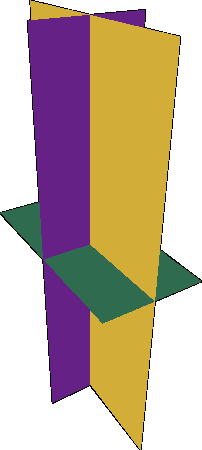
\includegraphics{asy/axesgraphic.pdf}}
  \put(9.5,-8.5){
\includegraphics{asy/shadow.pdf}}
  \put(15.25,-3){\makebox[0pt][r]{\frontcovertext{Linear Algebra}}}
  \put(15.25,-3.7){\makebox[0pt][r]{\frontcoverauthortext{Jim Hef{}feron}}}
  \put(15.25,-7.95){\makebox[0pt][r]{\frontcoverurltext{hefferon.net/linearalgebra}}}
  \put(15.25,-2.20){\makebox[0pt][r]{\frontcovereditiontext{Fourth edition}}}
  \put(7.65,-9.5){\spine}
  \put(1.0,-1.0){\backcoverhead}
  \put(1.0,-1.9){\backcovertext}

  \ifbool{showkdplinesbool}{% 
    % Front Cover width, height
    % Back cover
    \put(0.125,-0.125){\color{blue}\line(1,0){7.5}} % \FrontCoverWidth wide
      \put(0.125,-9.375){\color{blue}\line(1,0){7.5}} % \FrontCoverWidth wide
      \put(0.125,-0.125){\color{blue}\line(0,-1){9.25}} % \FrontCoverHeight tall
      \put(7.625,-0.125){\color{blue}\line(0,-1){9.25}}
    \put(0.25,-0.25){\color{blue}\line(1,0){7.375}} % \FrontCoverSafeWidth wide
      \put(0.25,-9.25){\color{blue}\line(1,0){7.375}} % \FrontCoverSafeWidth wide
      \put(0.25,-0.25){\color{blue}\line(0,-1){9.0}} % \FrontCoverSafeHeight tall
    % % Spine
    \put(7.687,-0.25){\color{blue}\line(1,0){1.071}} % 
      \put(7.687,-9.25){\color{blue}\line(1,0){1.071}} % 
    \put(7.687,-0.25){\color{blue}\line(0,-1){9}} %
      \put(8.758,-0.25){\color{blue}\line(0,-1){9}} %
    % % Front Cover
    \put(16.341,-0.125){\color{blue}\line(-1,0){7.5}} % 
      \put(16.341,-9.375){\color{blue}\line(-1,0){7.5}} % 
    \put(16.341,-0.125){\color{blue}\line(0,-1){9.25}} % 
      \put(8.821,-0.125){\color{blue}\line(0,-1){9.25}} % 
    \put(16.216,-0.25){\color{blue}\line(-1,0){7.375}} % Safe area
      \put(16.216,-9.25){\color{blue}\line(-1,0){7.375}} % 
    \put(16.216,-0.25){\color{blue}\line(0,-1){9}} % 
  }{}
\end{picture}
\end{document}
"
\ifdefined\showkdplines
  \booltrue{showkdplinesbool}
\fi
\ifbool{showkdplinesbool}{\typeout{!!! KDP LINES SHOWN}}{}

% Size of page
% Kindle Direct Publishing gives this for a 531 page book;
% see the graphic KDP_diagram_531_pages.png
% # 	Description 	Width (in) 	Height (in)
% 1 	Full Cover 	16.446 	9.5
% 2 	Front Cover 	7.5 	9.25
% 3 	Safe Area 	7.375 	9
% 4 	Bleed 	0.125 	0.125
% 5 	Margin 	0.125 	0.125
% 6 	Spine 	1.196 	9.25
% 7 	Spine Safe Area 	1.071 	9
% 8 	Spine Margin 	0.062 	0.062
% 9 	Barcode Margin 	0.25 	0.25 

% I could calculate some of these from the others, but why?
% Number 3
\newlength{\FrontCoverSafeWidth}
  \setlength{\FrontCoverSafeWidth}{7.375in}
\newlength{\FrontCoverSafeHeight}
  \setlength{\FrontCoverSafeHeight}{9in}
% Number 5
\newlength{\FrontCoverMarginWidth}
  \setlength{\FrontCoverMarginWidth}{0.125in}
\newlength{\FrontCoverMarginHeight}
  \setlength{\FrontCoverMarginHeight}{0.125in}
% Number 2
\newlength{\FrontCoverWidth}
  \setlength{\FrontCoverWidth}{7.5in}
\newlength{\FrontCoverHeight}
  \setlength{\FrontCoverHeight}{9.25in}
% Number 4
\newlength{\BleedWidth}
  \setlength{\BleedWidth}{0.125in}
\newlength{\BleedHeight}
  \setlength{\BleedHeight}{0.125in}
% Number 7
\newlength{\SpineSafeWidth}
  \setlength{\SpineSafeWidth}{1.071in}
\newlength{\SpineSafeHeight}
  \setlength{\SpineSafeHeight}{9.0in}
% Number 8
\newlength{\SpineMarginWidth}
  \setlength{\SpineMarginWidth}{0.062in}
\newlength{\SpineMarginHeight}
  \setlength{\SpineMarginHeight}{0.062in}
% Number 9
\newlength{\BarcodeMarginWidth}
  \setlength{\BarcodeMarginWidth}{0.25in}
\newlength{\BarcodeMarginHeight}
  \setlength{\BarcodeMarginHeight}{0.25in}
% Number 6
\newlength{\SpineWidth}
  \setlength{\SpineWidth}{7.375in}
\newlength{\SpineHeight}
  \setlength{\SpineHeight}{9in}
% Number 1
\newlength{\FullCoverWidth}
  \setlength{\FullCoverWidth}{16.446in}
\newlength{\FullCoverHeight}
  \setlength{\FullCoverHeight}{9.5in}

\newlength{\totalcoverwidth} \setlength{\totalcoverwidth}{15.0in} % 7.5+7.5
\newlength{\spinewidth} \setlength{\spinewidth}{1in}
\addtolength{\totalcoverwidth}{\spinewidth}
\usepackage[papersize={16.446in,10in},margin=0in]{geometry}  

% ==== Spine ========
% 
\newcommand{\spinetext}[1]{\color{black}\fontsize{38pt}{8pt}{\fontfamily{ugq}\selectfont #1}}
\newcommand{\spineauthortext}[1]{\color{coverdarkcolor}\fontsize{23pt}{8pt}{\fontfamily{ugq}\selectfont{#1}}}
\newcommand{\spine}{%
\setlength{\unitlength}{1in}
\begin{picture}(1,9.5)
  \setstackgap{S}{2.1ex}
  % \put(0.235,5.65){\Shortstack{{\spinetext{L}} {\spinetext{I}} {\spinetext{N}} {\spinetext{E}} {\spinetext{A}} {\spinetext{R}}}}
  \put(0.18,8.5){\rotatebox[origin=lc]{-90}{\spinetext{Linear Algebra}\hspace{2.15in}\spineauthortext{Hef{}feron}}}
  \setstackgap{S}{0.9ex}
  % \put(0.3925,1.15){\Shortstack{{\spineauthortext{H}{14}} {\spineauthortext{E}{14}} {\spineauthortext{F}{14}} {\spineauthortext{F}{14}} {\spineauthortext{E}{14}} {\spineauthortext{R}{14}} {\spineauthortext{O}{14}} {\spineauthortext{N}{14}}}} % tried fake small caps by making the H be 14 pt, others be 11
\end{picture}
}


% ==== Back cover ========
% 
\newcommand{\backcovertext}{%
\RaggedRight
\color{black}\fontsize{14pt}{17pt}\fontfamily{fos}\selectfont
\begin{minipage}[t]{5.75in}
\setlength{\parskip}{1.4ex}
This text covers a standard first course:
Gauss's Method, vector spaces, linear maps and matrices, determinants,
and eigenvalues and eigenvectors.
In addition, each chapter ends with some
brief topics, including applications.

What sets this book apart is careful motivation, 
many examples, and extensive exercise sets.
Together, these help each student master the material of
the course and also help an instructor develop their student's  
level of mathematical maturity.

This book
has been freely available online for many years. 
It is widely used, 
both in classrooms and for self-study.
It is supported by worked answers for all exercises, 
projection slides for classroom use, 
and a lab manual based on \textit{Sage}. 

\vspace{.2in}
\noindent\textbf{Winner of the Math Association of America's Solow Award:}\\[1.35ex]
\vspace{-.225in}
\begin{center}
\parbox{5.5in}{
``The clear writing style, tremendous variety of exercises,
amenability to use with active learning strategies, and the
careful attention to detail in preparation mean that the text
is exceptionally adaptable.''}
\end{center}
\end{minipage}
}

\newcommand{\backcoverhead}{%
\setlength{\unitlength}{1in}
\begin{picture}(0,0)
  % \put(1,-.1){{\color{coverbgcolor}\rule{4.4in}{2pt}}}
  \put(0,-.1){{\color{coverbgcolor}\rule{5.05in}{2pt}}}
  \put(0.0,0){\color{coverboldcolor}\fontsize{25pt}{8pt}\fontfamily{fos}\selectfont \textit{A developmental approach to}}
  \put(3.0,-.45){\color{black}\fontsize{25pt}{8pt}\fontfamily{fos}\selectfont \textbf{Linear Algebra}}
\end{picture}
}




% ==== Front cover ========
% 
\newcommand{\frontcovertext}[1]{\color{black}\fontsize{55pt}{8pt}{\fontfamily{ugq}\selectfont #1}}
% \newcommand{\frontcovereditiontext}[1]{\color{black}\fontsize{20pt}{8pt}{\fontfamily{ugq}\selectfont #1}}
\newcommand{\frontcovereditiontext}[1]{\color[gray]{0.4}\fontsize{20pt}{6pt}\fontfamily{ugq}\selectfont \textsf{#1}}
% \newcommand{\frontcovereditiontext}[1]{\color{black}\fontsize{20pt}{6pt}\fontfamily{ugq}\selectfont #1}
\newcommand{\frontcoverauthortext}[1]{\color{black}\fontsize{27.5pt}{6pt}{\fontfamily{ugq}\selectfont #1}}
\newcommand{\frontcoverurltext}[1]{\color[gray]{0.4}\fontsize{18pt}{6pt}\fontfamily{ugq}\selectfont \textsf{#1}}
% \newcommand{\frontcoverurltext}[1]{\color[gray]{0.4}{\lato \fontsize{18pt}{6pt}\fontseries{sb}\selectfont #1}}


\setlength{\parindent}{0in}
\begin{document}\pagestyle{empty}\thispagestyle{empty}

\setlength{\unitlength}{1in}
\begin{picture}(0,0) 
  \ifbool{showguidelinesbool}{% 
    \put(0,-1){\makebox[0in]{\color{red}0}}
    \put(1,-1){\makebox[0in]{\color{red}1}}
    \put(2,-1){\makebox[0in]{\color{red}2}}
    \put(3,-1){\makebox[0in]{\color{red}3}}
    \put(4,-1){\makebox[0in]{\color{red}4}}
    \put(5,-1){\makebox[0in]{\color{red}5}}
    \put(6,-1){\makebox[0in]{\color{red}6}}
    \put(7,-1){\makebox[0in]{\color{red}7}}
    \put(7.5,-1){\color{red}\line(0,-1){8}}
    \put(8,-1){\makebox[0in]{\color{red}8}}
    \put(8,-1){\color{blue}\line(0,-1){8}}
    \put(8.5,-1){\color{red}\line(0,-1){8}}
    \put(9,-1){\makebox[0in]{\color{red}9}}
    \put(9.5,-1){\color{blue}\line(0,-1){8}}
    \put(10,-1){\makebox[0in]{\color{red}10}}
    \put(11,-1){\makebox[0in]{\color{red}11}}
    \put(12,-1){\makebox[0in]{\color{red}12}}
    \put(13,-1){\makebox[0in]{\color{red}13}}
    \put(14,-1){\makebox[0in]{\color{red}14}}
    \put(15,-1){\makebox[0in]{\color{red}15}}
    \put(15,-1){\color{blue}\line(0,-1){8}}
    \put(16,-1){\makebox[0in]{\color{red}16}}
  }{} 

  \put(9.5,-7.57){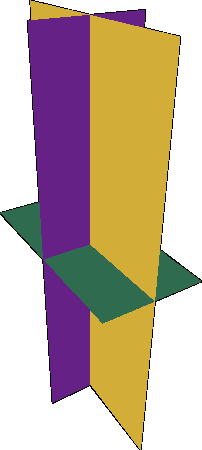
\includegraphics{asy/axesgraphic.pdf}}
  \put(9.5,-8.5){
\includegraphics{asy/shadow.pdf}}
  \put(15.25,-3){\makebox[0pt][r]{\frontcovertext{Linear Algebra}}}
  \put(15.25,-3.7){\makebox[0pt][r]{\frontcoverauthortext{Jim Hef{}feron}}}
  \put(15.25,-7.95){\makebox[0pt][r]{\frontcoverurltext{hefferon.net/linearalgebra}}}
  \put(15.25,-2.20){\makebox[0pt][r]{\frontcovereditiontext{Fourth edition}}}
  \put(7.65,-9.5){\spine}
  \put(1.0,-1.0){\backcoverhead}
  \put(1.0,-1.9){\backcovertext}

  \ifbool{showkdplinesbool}{% 
    % Front Cover width, height
    % Back cover
    \put(0.125,-0.125){\color{blue}\line(1,0){7.5}} % \FrontCoverWidth wide
      \put(0.125,-9.375){\color{blue}\line(1,0){7.5}} % \FrontCoverWidth wide
      \put(0.125,-0.125){\color{blue}\line(0,-1){9.25}} % \FrontCoverHeight tall
      \put(7.625,-0.125){\color{blue}\line(0,-1){9.25}}
    \put(0.25,-0.25){\color{blue}\line(1,0){7.375}} % \FrontCoverSafeWidth wide
      \put(0.25,-9.25){\color{blue}\line(1,0){7.375}} % \FrontCoverSafeWidth wide
      \put(0.25,-0.25){\color{blue}\line(0,-1){9.0}} % \FrontCoverSafeHeight tall
    % % Spine
    \put(7.687,-0.25){\color{blue}\line(1,0){1.071}} % 
      \put(7.687,-9.25){\color{blue}\line(1,0){1.071}} % 
    \put(7.687,-0.25){\color{blue}\line(0,-1){9}} %
      \put(8.758,-0.25){\color{blue}\line(0,-1){9}} %
    % % Front Cover
    \put(16.341,-0.125){\color{blue}\line(-1,0){7.5}} % 
      \put(16.341,-9.375){\color{blue}\line(-1,0){7.5}} % 
    \put(16.341,-0.125){\color{blue}\line(0,-1){9.25}} % 
      \put(8.821,-0.125){\color{blue}\line(0,-1){9.25}} % 
    \put(16.216,-0.25){\color{blue}\line(-1,0){7.375}} % Safe area
      \put(16.216,-9.25){\color{blue}\line(-1,0){7.375}} % 
    \put(16.216,-0.25){\color{blue}\line(0,-1){9}} % 
  }{}
\end{picture}
\end{document}
"
% See http://stackoverflow.com/a/1466610
\ifdefined\showguidelines
  \booltrue{showguidelinesbool}
\fi
\ifbool{showguidelinesbool}{\typeout{!!! GUIDELINES SHOWN}}{}
% Guidelines to show KDP lines.  Show or not?
\newbool{showkdplinesbool}
  % set the default by uncommenting one or the other
  \booltrue{showkdplinesbool} 
  % \boolfalse{showkdplinesbool}  
% You can cause KDP lines to be shown by invoking with
%   pdflatex "\def\showkdplines{}\documentclass{article}
% \usepackage{covergraphic}
\usepackage{graphicx}
\usepackage{ragged2e}
\usepackage{xcolor}
\colorlet{coverdarkcolor}{black}
\definecolor{coverbgcolor}{RGB}{212,175,55}  % gold
\definecolor{coverboldcolor}{RGB}{0,67,37}  % green
% \definecolor{coverboldcolor}{RGB}{103,0,153}  % purple

\usepackage[defaultsans]{lato}

\usepackage{stackengine}
\renewcommand{\stackalignment}{c}

% I want the booleans offered by this package
\usepackage{etoolbox}
% Guidelines help to arrange the parts visually.  Show or not?
\newbool{showguidelinesbool}
  % set the default by uncommenting one or the other
  % \booltrue{showguidelinesbool} 
  \boolfalse{showguidelinesbool}  
% You can cause guidelines to be shown by invoking with
%   pdflatex "\def\showguidelines{}\documentclass{article}
% \usepackage{covergraphic}
\usepackage{graphicx}
\usepackage{ragged2e}
\usepackage{xcolor}
\colorlet{coverdarkcolor}{black}
\definecolor{coverbgcolor}{RGB}{212,175,55}  % gold
\definecolor{coverboldcolor}{RGB}{0,67,37}  % green
% \definecolor{coverboldcolor}{RGB}{103,0,153}  % purple

\usepackage[defaultsans]{lato}

\usepackage{stackengine}
\renewcommand{\stackalignment}{c}

% I want the booleans offered by this package
\usepackage{etoolbox}
% Guidelines help to arrange the parts visually.  Show or not?
\newbool{showguidelinesbool}
  % set the default by uncommenting one or the other
  % \booltrue{showguidelinesbool} 
  \boolfalse{showguidelinesbool}  
% You can cause guidelines to be shown by invoking with
%   pdflatex "\def\showguidelines{}\input{cover}"
% See http://stackoverflow.com/a/1466610
\ifdefined\showguidelines
  \booltrue{showguidelinesbool}
\fi
\ifbool{showguidelinesbool}{\typeout{!!! GUIDELINES SHOWN}}{}
% Guidelines to show KDP lines.  Show or not?
\newbool{showkdplinesbool}
  % set the default by uncommenting one or the other
  \booltrue{showkdplinesbool} 
  % \boolfalse{showkdplinesbool}  
% You can cause KDP lines to be shown by invoking with
%   pdflatex "\def\showkdplines{}\input{cover}"
\ifdefined\showkdplines
  \booltrue{showkdplinesbool}
\fi
\ifbool{showkdplinesbool}{\typeout{!!! KDP LINES SHOWN}}{}

% Size of page
% Kindle Direct Publishing gives this for a 531 page book;
% see the graphic KDP_diagram_531_pages.png
% # 	Description 	Width (in) 	Height (in)
% 1 	Full Cover 	16.446 	9.5
% 2 	Front Cover 	7.5 	9.25
% 3 	Safe Area 	7.375 	9
% 4 	Bleed 	0.125 	0.125
% 5 	Margin 	0.125 	0.125
% 6 	Spine 	1.196 	9.25
% 7 	Spine Safe Area 	1.071 	9
% 8 	Spine Margin 	0.062 	0.062
% 9 	Barcode Margin 	0.25 	0.25 

% I could calculate some of these from the others, but why?
% Number 3
\newlength{\FrontCoverSafeWidth}
  \setlength{\FrontCoverSafeWidth}{7.375in}
\newlength{\FrontCoverSafeHeight}
  \setlength{\FrontCoverSafeHeight}{9in}
% Number 5
\newlength{\FrontCoverMarginWidth}
  \setlength{\FrontCoverMarginWidth}{0.125in}
\newlength{\FrontCoverMarginHeight}
  \setlength{\FrontCoverMarginHeight}{0.125in}
% Number 2
\newlength{\FrontCoverWidth}
  \setlength{\FrontCoverWidth}{7.5in}
\newlength{\FrontCoverHeight}
  \setlength{\FrontCoverHeight}{9.25in}
% Number 4
\newlength{\BleedWidth}
  \setlength{\BleedWidth}{0.125in}
\newlength{\BleedHeight}
  \setlength{\BleedHeight}{0.125in}
% Number 7
\newlength{\SpineSafeWidth}
  \setlength{\SpineSafeWidth}{1.071in}
\newlength{\SpineSafeHeight}
  \setlength{\SpineSafeHeight}{9.0in}
% Number 8
\newlength{\SpineMarginWidth}
  \setlength{\SpineMarginWidth}{0.062in}
\newlength{\SpineMarginHeight}
  \setlength{\SpineMarginHeight}{0.062in}
% Number 9
\newlength{\BarcodeMarginWidth}
  \setlength{\BarcodeMarginWidth}{0.25in}
\newlength{\BarcodeMarginHeight}
  \setlength{\BarcodeMarginHeight}{0.25in}
% Number 6
\newlength{\SpineWidth}
  \setlength{\SpineWidth}{7.375in}
\newlength{\SpineHeight}
  \setlength{\SpineHeight}{9in}
% Number 1
\newlength{\FullCoverWidth}
  \setlength{\FullCoverWidth}{16.446in}
\newlength{\FullCoverHeight}
  \setlength{\FullCoverHeight}{9.5in}

\newlength{\totalcoverwidth} \setlength{\totalcoverwidth}{15.0in} % 7.5+7.5
\newlength{\spinewidth} \setlength{\spinewidth}{1in}
\addtolength{\totalcoverwidth}{\spinewidth}
\usepackage[papersize={16.446in,10in},margin=0in]{geometry}  

% ==== Spine ========
% 
\newcommand{\spinetext}[1]{\color{black}\fontsize{38pt}{8pt}{\fontfamily{ugq}\selectfont #1}}
\newcommand{\spineauthortext}[1]{\color{coverdarkcolor}\fontsize{23pt}{8pt}{\fontfamily{ugq}\selectfont{#1}}}
\newcommand{\spine}{%
\setlength{\unitlength}{1in}
\begin{picture}(1,9.5)
  \setstackgap{S}{2.1ex}
  % \put(0.235,5.65){\Shortstack{{\spinetext{L}} {\spinetext{I}} {\spinetext{N}} {\spinetext{E}} {\spinetext{A}} {\spinetext{R}}}}
  \put(0.18,8.5){\rotatebox[origin=lc]{-90}{\spinetext{Linear Algebra}\hspace{2.15in}\spineauthortext{Hef{}feron}}}
  \setstackgap{S}{0.9ex}
  % \put(0.3925,1.15){\Shortstack{{\spineauthortext{H}{14}} {\spineauthortext{E}{14}} {\spineauthortext{F}{14}} {\spineauthortext{F}{14}} {\spineauthortext{E}{14}} {\spineauthortext{R}{14}} {\spineauthortext{O}{14}} {\spineauthortext{N}{14}}}} % tried fake small caps by making the H be 14 pt, others be 11
\end{picture}
}


% ==== Back cover ========
% 
\newcommand{\backcovertext}{%
\RaggedRight
\color{black}\fontsize{14pt}{17pt}\fontfamily{fos}\selectfont
\begin{minipage}[t]{5.75in}
\setlength{\parskip}{1.4ex}
This text covers a standard first course:
Gauss's Method, vector spaces, linear maps and matrices, determinants,
and eigenvalues and eigenvectors.
In addition, each chapter ends with some
brief topics, including applications.

What sets this book apart is careful motivation, 
many examples, and extensive exercise sets.
Together, these help each student master the material of
the course and also help an instructor develop their student's  
level of mathematical maturity.

This book
has been freely available online for many years. 
It is widely used, 
both in classrooms and for self-study.
It is supported by worked answers for all exercises, 
projection slides for classroom use, 
and a lab manual based on \textit{Sage}. 

\vspace{.2in}
\noindent\textbf{Winner of the Math Association of America's Solow Award:}\\[1.35ex]
\vspace{-.225in}
\begin{center}
\parbox{5.5in}{
``The clear writing style, tremendous variety of exercises,
amenability to use with active learning strategies, and the
careful attention to detail in preparation mean that the text
is exceptionally adaptable.''}
\end{center}
\end{minipage}
}

\newcommand{\backcoverhead}{%
\setlength{\unitlength}{1in}
\begin{picture}(0,0)
  % \put(1,-.1){{\color{coverbgcolor}\rule{4.4in}{2pt}}}
  \put(0,-.1){{\color{coverbgcolor}\rule{5.05in}{2pt}}}
  \put(0.0,0){\color{coverboldcolor}\fontsize{25pt}{8pt}\fontfamily{fos}\selectfont \textit{A developmental approach to}}
  \put(3.0,-.45){\color{black}\fontsize{25pt}{8pt}\fontfamily{fos}\selectfont \textbf{Linear Algebra}}
\end{picture}
}




% ==== Front cover ========
% 
\newcommand{\frontcovertext}[1]{\color{black}\fontsize{55pt}{8pt}{\fontfamily{ugq}\selectfont #1}}
% \newcommand{\frontcovereditiontext}[1]{\color{black}\fontsize{20pt}{8pt}{\fontfamily{ugq}\selectfont #1}}
\newcommand{\frontcovereditiontext}[1]{\color[gray]{0.4}\fontsize{20pt}{6pt}\fontfamily{ugq}\selectfont \textsf{#1}}
% \newcommand{\frontcovereditiontext}[1]{\color{black}\fontsize{20pt}{6pt}\fontfamily{ugq}\selectfont #1}
\newcommand{\frontcoverauthortext}[1]{\color{black}\fontsize{27.5pt}{6pt}{\fontfamily{ugq}\selectfont #1}}
\newcommand{\frontcoverurltext}[1]{\color[gray]{0.4}\fontsize{18pt}{6pt}\fontfamily{ugq}\selectfont \textsf{#1}}
% \newcommand{\frontcoverurltext}[1]{\color[gray]{0.4}{\lato \fontsize{18pt}{6pt}\fontseries{sb}\selectfont #1}}


\setlength{\parindent}{0in}
\begin{document}\pagestyle{empty}\thispagestyle{empty}

\setlength{\unitlength}{1in}
\begin{picture}(0,0) 
  \ifbool{showguidelinesbool}{% 
    \put(0,-1){\makebox[0in]{\color{red}0}}
    \put(1,-1){\makebox[0in]{\color{red}1}}
    \put(2,-1){\makebox[0in]{\color{red}2}}
    \put(3,-1){\makebox[0in]{\color{red}3}}
    \put(4,-1){\makebox[0in]{\color{red}4}}
    \put(5,-1){\makebox[0in]{\color{red}5}}
    \put(6,-1){\makebox[0in]{\color{red}6}}
    \put(7,-1){\makebox[0in]{\color{red}7}}
    \put(7.5,-1){\color{red}\line(0,-1){8}}
    \put(8,-1){\makebox[0in]{\color{red}8}}
    \put(8,-1){\color{blue}\line(0,-1){8}}
    \put(8.5,-1){\color{red}\line(0,-1){8}}
    \put(9,-1){\makebox[0in]{\color{red}9}}
    \put(9.5,-1){\color{blue}\line(0,-1){8}}
    \put(10,-1){\makebox[0in]{\color{red}10}}
    \put(11,-1){\makebox[0in]{\color{red}11}}
    \put(12,-1){\makebox[0in]{\color{red}12}}
    \put(13,-1){\makebox[0in]{\color{red}13}}
    \put(14,-1){\makebox[0in]{\color{red}14}}
    \put(15,-1){\makebox[0in]{\color{red}15}}
    \put(15,-1){\color{blue}\line(0,-1){8}}
    \put(16,-1){\makebox[0in]{\color{red}16}}
  }{} 

  \put(9.5,-7.57){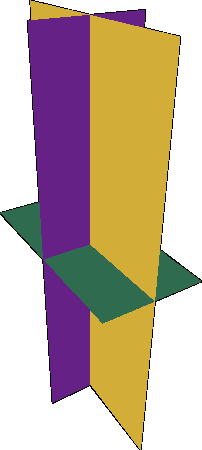
\includegraphics{asy/axesgraphic.pdf}}
  \put(9.5,-8.5){
\includegraphics{asy/shadow.pdf}}
  \put(15.25,-3){\makebox[0pt][r]{\frontcovertext{Linear Algebra}}}
  \put(15.25,-3.7){\makebox[0pt][r]{\frontcoverauthortext{Jim Hef{}feron}}}
  \put(15.25,-7.95){\makebox[0pt][r]{\frontcoverurltext{hefferon.net/linearalgebra}}}
  \put(15.25,-2.20){\makebox[0pt][r]{\frontcovereditiontext{Fourth edition}}}
  \put(7.65,-9.5){\spine}
  \put(1.0,-1.0){\backcoverhead}
  \put(1.0,-1.9){\backcovertext}

  \ifbool{showkdplinesbool}{% 
    % Front Cover width, height
    % Back cover
    \put(0.125,-0.125){\color{blue}\line(1,0){7.5}} % \FrontCoverWidth wide
      \put(0.125,-9.375){\color{blue}\line(1,0){7.5}} % \FrontCoverWidth wide
      \put(0.125,-0.125){\color{blue}\line(0,-1){9.25}} % \FrontCoverHeight tall
      \put(7.625,-0.125){\color{blue}\line(0,-1){9.25}}
    \put(0.25,-0.25){\color{blue}\line(1,0){7.375}} % \FrontCoverSafeWidth wide
      \put(0.25,-9.25){\color{blue}\line(1,0){7.375}} % \FrontCoverSafeWidth wide
      \put(0.25,-0.25){\color{blue}\line(0,-1){9.0}} % \FrontCoverSafeHeight tall
    % % Spine
    \put(7.687,-0.25){\color{blue}\line(1,0){1.071}} % 
      \put(7.687,-9.25){\color{blue}\line(1,0){1.071}} % 
    \put(7.687,-0.25){\color{blue}\line(0,-1){9}} %
      \put(8.758,-0.25){\color{blue}\line(0,-1){9}} %
    % % Front Cover
    \put(16.341,-0.125){\color{blue}\line(-1,0){7.5}} % 
      \put(16.341,-9.375){\color{blue}\line(-1,0){7.5}} % 
    \put(16.341,-0.125){\color{blue}\line(0,-1){9.25}} % 
      \put(8.821,-0.125){\color{blue}\line(0,-1){9.25}} % 
    \put(16.216,-0.25){\color{blue}\line(-1,0){7.375}} % Safe area
      \put(16.216,-9.25){\color{blue}\line(-1,0){7.375}} % 
    \put(16.216,-0.25){\color{blue}\line(0,-1){9}} % 
  }{}
\end{picture}
\end{document}
"
% See http://stackoverflow.com/a/1466610
\ifdefined\showguidelines
  \booltrue{showguidelinesbool}
\fi
\ifbool{showguidelinesbool}{\typeout{!!! GUIDELINES SHOWN}}{}
% Guidelines to show KDP lines.  Show or not?
\newbool{showkdplinesbool}
  % set the default by uncommenting one or the other
  \booltrue{showkdplinesbool} 
  % \boolfalse{showkdplinesbool}  
% You can cause KDP lines to be shown by invoking with
%   pdflatex "\def\showkdplines{}\documentclass{article}
% \usepackage{covergraphic}
\usepackage{graphicx}
\usepackage{ragged2e}
\usepackage{xcolor}
\colorlet{coverdarkcolor}{black}
\definecolor{coverbgcolor}{RGB}{212,175,55}  % gold
\definecolor{coverboldcolor}{RGB}{0,67,37}  % green
% \definecolor{coverboldcolor}{RGB}{103,0,153}  % purple

\usepackage[defaultsans]{lato}

\usepackage{stackengine}
\renewcommand{\stackalignment}{c}

% I want the booleans offered by this package
\usepackage{etoolbox}
% Guidelines help to arrange the parts visually.  Show or not?
\newbool{showguidelinesbool}
  % set the default by uncommenting one or the other
  % \booltrue{showguidelinesbool} 
  \boolfalse{showguidelinesbool}  
% You can cause guidelines to be shown by invoking with
%   pdflatex "\def\showguidelines{}\input{cover}"
% See http://stackoverflow.com/a/1466610
\ifdefined\showguidelines
  \booltrue{showguidelinesbool}
\fi
\ifbool{showguidelinesbool}{\typeout{!!! GUIDELINES SHOWN}}{}
% Guidelines to show KDP lines.  Show or not?
\newbool{showkdplinesbool}
  % set the default by uncommenting one or the other
  \booltrue{showkdplinesbool} 
  % \boolfalse{showkdplinesbool}  
% You can cause KDP lines to be shown by invoking with
%   pdflatex "\def\showkdplines{}\input{cover}"
\ifdefined\showkdplines
  \booltrue{showkdplinesbool}
\fi
\ifbool{showkdplinesbool}{\typeout{!!! KDP LINES SHOWN}}{}

% Size of page
% Kindle Direct Publishing gives this for a 531 page book;
% see the graphic KDP_diagram_531_pages.png
% # 	Description 	Width (in) 	Height (in)
% 1 	Full Cover 	16.446 	9.5
% 2 	Front Cover 	7.5 	9.25
% 3 	Safe Area 	7.375 	9
% 4 	Bleed 	0.125 	0.125
% 5 	Margin 	0.125 	0.125
% 6 	Spine 	1.196 	9.25
% 7 	Spine Safe Area 	1.071 	9
% 8 	Spine Margin 	0.062 	0.062
% 9 	Barcode Margin 	0.25 	0.25 

% I could calculate some of these from the others, but why?
% Number 3
\newlength{\FrontCoverSafeWidth}
  \setlength{\FrontCoverSafeWidth}{7.375in}
\newlength{\FrontCoverSafeHeight}
  \setlength{\FrontCoverSafeHeight}{9in}
% Number 5
\newlength{\FrontCoverMarginWidth}
  \setlength{\FrontCoverMarginWidth}{0.125in}
\newlength{\FrontCoverMarginHeight}
  \setlength{\FrontCoverMarginHeight}{0.125in}
% Number 2
\newlength{\FrontCoverWidth}
  \setlength{\FrontCoverWidth}{7.5in}
\newlength{\FrontCoverHeight}
  \setlength{\FrontCoverHeight}{9.25in}
% Number 4
\newlength{\BleedWidth}
  \setlength{\BleedWidth}{0.125in}
\newlength{\BleedHeight}
  \setlength{\BleedHeight}{0.125in}
% Number 7
\newlength{\SpineSafeWidth}
  \setlength{\SpineSafeWidth}{1.071in}
\newlength{\SpineSafeHeight}
  \setlength{\SpineSafeHeight}{9.0in}
% Number 8
\newlength{\SpineMarginWidth}
  \setlength{\SpineMarginWidth}{0.062in}
\newlength{\SpineMarginHeight}
  \setlength{\SpineMarginHeight}{0.062in}
% Number 9
\newlength{\BarcodeMarginWidth}
  \setlength{\BarcodeMarginWidth}{0.25in}
\newlength{\BarcodeMarginHeight}
  \setlength{\BarcodeMarginHeight}{0.25in}
% Number 6
\newlength{\SpineWidth}
  \setlength{\SpineWidth}{7.375in}
\newlength{\SpineHeight}
  \setlength{\SpineHeight}{9in}
% Number 1
\newlength{\FullCoverWidth}
  \setlength{\FullCoverWidth}{16.446in}
\newlength{\FullCoverHeight}
  \setlength{\FullCoverHeight}{9.5in}

\newlength{\totalcoverwidth} \setlength{\totalcoverwidth}{15.0in} % 7.5+7.5
\newlength{\spinewidth} \setlength{\spinewidth}{1in}
\addtolength{\totalcoverwidth}{\spinewidth}
\usepackage[papersize={16.446in,10in},margin=0in]{geometry}  

% ==== Spine ========
% 
\newcommand{\spinetext}[1]{\color{black}\fontsize{38pt}{8pt}{\fontfamily{ugq}\selectfont #1}}
\newcommand{\spineauthortext}[1]{\color{coverdarkcolor}\fontsize{23pt}{8pt}{\fontfamily{ugq}\selectfont{#1}}}
\newcommand{\spine}{%
\setlength{\unitlength}{1in}
\begin{picture}(1,9.5)
  \setstackgap{S}{2.1ex}
  % \put(0.235,5.65){\Shortstack{{\spinetext{L}} {\spinetext{I}} {\spinetext{N}} {\spinetext{E}} {\spinetext{A}} {\spinetext{R}}}}
  \put(0.18,8.5){\rotatebox[origin=lc]{-90}{\spinetext{Linear Algebra}\hspace{2.15in}\spineauthortext{Hef{}feron}}}
  \setstackgap{S}{0.9ex}
  % \put(0.3925,1.15){\Shortstack{{\spineauthortext{H}{14}} {\spineauthortext{E}{14}} {\spineauthortext{F}{14}} {\spineauthortext{F}{14}} {\spineauthortext{E}{14}} {\spineauthortext{R}{14}} {\spineauthortext{O}{14}} {\spineauthortext{N}{14}}}} % tried fake small caps by making the H be 14 pt, others be 11
\end{picture}
}


% ==== Back cover ========
% 
\newcommand{\backcovertext}{%
\RaggedRight
\color{black}\fontsize{14pt}{17pt}\fontfamily{fos}\selectfont
\begin{minipage}[t]{5.75in}
\setlength{\parskip}{1.4ex}
This text covers a standard first course:
Gauss's Method, vector spaces, linear maps and matrices, determinants,
and eigenvalues and eigenvectors.
In addition, each chapter ends with some
brief topics, including applications.

What sets this book apart is careful motivation, 
many examples, and extensive exercise sets.
Together, these help each student master the material of
the course and also help an instructor develop their student's  
level of mathematical maturity.

This book
has been freely available online for many years. 
It is widely used, 
both in classrooms and for self-study.
It is supported by worked answers for all exercises, 
projection slides for classroom use, 
and a lab manual based on \textit{Sage}. 

\vspace{.2in}
\noindent\textbf{Winner of the Math Association of America's Solow Award:}\\[1.35ex]
\vspace{-.225in}
\begin{center}
\parbox{5.5in}{
``The clear writing style, tremendous variety of exercises,
amenability to use with active learning strategies, and the
careful attention to detail in preparation mean that the text
is exceptionally adaptable.''}
\end{center}
\end{minipage}
}

\newcommand{\backcoverhead}{%
\setlength{\unitlength}{1in}
\begin{picture}(0,0)
  % \put(1,-.1){{\color{coverbgcolor}\rule{4.4in}{2pt}}}
  \put(0,-.1){{\color{coverbgcolor}\rule{5.05in}{2pt}}}
  \put(0.0,0){\color{coverboldcolor}\fontsize{25pt}{8pt}\fontfamily{fos}\selectfont \textit{A developmental approach to}}
  \put(3.0,-.45){\color{black}\fontsize{25pt}{8pt}\fontfamily{fos}\selectfont \textbf{Linear Algebra}}
\end{picture}
}




% ==== Front cover ========
% 
\newcommand{\frontcovertext}[1]{\color{black}\fontsize{55pt}{8pt}{\fontfamily{ugq}\selectfont #1}}
% \newcommand{\frontcovereditiontext}[1]{\color{black}\fontsize{20pt}{8pt}{\fontfamily{ugq}\selectfont #1}}
\newcommand{\frontcovereditiontext}[1]{\color[gray]{0.4}\fontsize{20pt}{6pt}\fontfamily{ugq}\selectfont \textsf{#1}}
% \newcommand{\frontcovereditiontext}[1]{\color{black}\fontsize{20pt}{6pt}\fontfamily{ugq}\selectfont #1}
\newcommand{\frontcoverauthortext}[1]{\color{black}\fontsize{27.5pt}{6pt}{\fontfamily{ugq}\selectfont #1}}
\newcommand{\frontcoverurltext}[1]{\color[gray]{0.4}\fontsize{18pt}{6pt}\fontfamily{ugq}\selectfont \textsf{#1}}
% \newcommand{\frontcoverurltext}[1]{\color[gray]{0.4}{\lato \fontsize{18pt}{6pt}\fontseries{sb}\selectfont #1}}


\setlength{\parindent}{0in}
\begin{document}\pagestyle{empty}\thispagestyle{empty}

\setlength{\unitlength}{1in}
\begin{picture}(0,0) 
  \ifbool{showguidelinesbool}{% 
    \put(0,-1){\makebox[0in]{\color{red}0}}
    \put(1,-1){\makebox[0in]{\color{red}1}}
    \put(2,-1){\makebox[0in]{\color{red}2}}
    \put(3,-1){\makebox[0in]{\color{red}3}}
    \put(4,-1){\makebox[0in]{\color{red}4}}
    \put(5,-1){\makebox[0in]{\color{red}5}}
    \put(6,-1){\makebox[0in]{\color{red}6}}
    \put(7,-1){\makebox[0in]{\color{red}7}}
    \put(7.5,-1){\color{red}\line(0,-1){8}}
    \put(8,-1){\makebox[0in]{\color{red}8}}
    \put(8,-1){\color{blue}\line(0,-1){8}}
    \put(8.5,-1){\color{red}\line(0,-1){8}}
    \put(9,-1){\makebox[0in]{\color{red}9}}
    \put(9.5,-1){\color{blue}\line(0,-1){8}}
    \put(10,-1){\makebox[0in]{\color{red}10}}
    \put(11,-1){\makebox[0in]{\color{red}11}}
    \put(12,-1){\makebox[0in]{\color{red}12}}
    \put(13,-1){\makebox[0in]{\color{red}13}}
    \put(14,-1){\makebox[0in]{\color{red}14}}
    \put(15,-1){\makebox[0in]{\color{red}15}}
    \put(15,-1){\color{blue}\line(0,-1){8}}
    \put(16,-1){\makebox[0in]{\color{red}16}}
  }{} 

  \put(9.5,-7.57){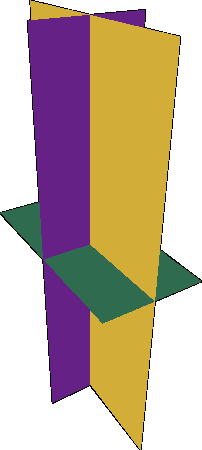
\includegraphics{asy/axesgraphic.pdf}}
  \put(9.5,-8.5){
\includegraphics{asy/shadow.pdf}}
  \put(15.25,-3){\makebox[0pt][r]{\frontcovertext{Linear Algebra}}}
  \put(15.25,-3.7){\makebox[0pt][r]{\frontcoverauthortext{Jim Hef{}feron}}}
  \put(15.25,-7.95){\makebox[0pt][r]{\frontcoverurltext{hefferon.net/linearalgebra}}}
  \put(15.25,-2.20){\makebox[0pt][r]{\frontcovereditiontext{Fourth edition}}}
  \put(7.65,-9.5){\spine}
  \put(1.0,-1.0){\backcoverhead}
  \put(1.0,-1.9){\backcovertext}

  \ifbool{showkdplinesbool}{% 
    % Front Cover width, height
    % Back cover
    \put(0.125,-0.125){\color{blue}\line(1,0){7.5}} % \FrontCoverWidth wide
      \put(0.125,-9.375){\color{blue}\line(1,0){7.5}} % \FrontCoverWidth wide
      \put(0.125,-0.125){\color{blue}\line(0,-1){9.25}} % \FrontCoverHeight tall
      \put(7.625,-0.125){\color{blue}\line(0,-1){9.25}}
    \put(0.25,-0.25){\color{blue}\line(1,0){7.375}} % \FrontCoverSafeWidth wide
      \put(0.25,-9.25){\color{blue}\line(1,0){7.375}} % \FrontCoverSafeWidth wide
      \put(0.25,-0.25){\color{blue}\line(0,-1){9.0}} % \FrontCoverSafeHeight tall
    % % Spine
    \put(7.687,-0.25){\color{blue}\line(1,0){1.071}} % 
      \put(7.687,-9.25){\color{blue}\line(1,0){1.071}} % 
    \put(7.687,-0.25){\color{blue}\line(0,-1){9}} %
      \put(8.758,-0.25){\color{blue}\line(0,-1){9}} %
    % % Front Cover
    \put(16.341,-0.125){\color{blue}\line(-1,0){7.5}} % 
      \put(16.341,-9.375){\color{blue}\line(-1,0){7.5}} % 
    \put(16.341,-0.125){\color{blue}\line(0,-1){9.25}} % 
      \put(8.821,-0.125){\color{blue}\line(0,-1){9.25}} % 
    \put(16.216,-0.25){\color{blue}\line(-1,0){7.375}} % Safe area
      \put(16.216,-9.25){\color{blue}\line(-1,0){7.375}} % 
    \put(16.216,-0.25){\color{blue}\line(0,-1){9}} % 
  }{}
\end{picture}
\end{document}
"
\ifdefined\showkdplines
  \booltrue{showkdplinesbool}
\fi
\ifbool{showkdplinesbool}{\typeout{!!! KDP LINES SHOWN}}{}

% Size of page
% Kindle Direct Publishing gives this for a 531 page book;
% see the graphic KDP_diagram_531_pages.png
% # 	Description 	Width (in) 	Height (in)
% 1 	Full Cover 	16.446 	9.5
% 2 	Front Cover 	7.5 	9.25
% 3 	Safe Area 	7.375 	9
% 4 	Bleed 	0.125 	0.125
% 5 	Margin 	0.125 	0.125
% 6 	Spine 	1.196 	9.25
% 7 	Spine Safe Area 	1.071 	9
% 8 	Spine Margin 	0.062 	0.062
% 9 	Barcode Margin 	0.25 	0.25 

% I could calculate some of these from the others, but why?
% Number 3
\newlength{\FrontCoverSafeWidth}
  \setlength{\FrontCoverSafeWidth}{7.375in}
\newlength{\FrontCoverSafeHeight}
  \setlength{\FrontCoverSafeHeight}{9in}
% Number 5
\newlength{\FrontCoverMarginWidth}
  \setlength{\FrontCoverMarginWidth}{0.125in}
\newlength{\FrontCoverMarginHeight}
  \setlength{\FrontCoverMarginHeight}{0.125in}
% Number 2
\newlength{\FrontCoverWidth}
  \setlength{\FrontCoverWidth}{7.5in}
\newlength{\FrontCoverHeight}
  \setlength{\FrontCoverHeight}{9.25in}
% Number 4
\newlength{\BleedWidth}
  \setlength{\BleedWidth}{0.125in}
\newlength{\BleedHeight}
  \setlength{\BleedHeight}{0.125in}
% Number 7
\newlength{\SpineSafeWidth}
  \setlength{\SpineSafeWidth}{1.071in}
\newlength{\SpineSafeHeight}
  \setlength{\SpineSafeHeight}{9.0in}
% Number 8
\newlength{\SpineMarginWidth}
  \setlength{\SpineMarginWidth}{0.062in}
\newlength{\SpineMarginHeight}
  \setlength{\SpineMarginHeight}{0.062in}
% Number 9
\newlength{\BarcodeMarginWidth}
  \setlength{\BarcodeMarginWidth}{0.25in}
\newlength{\BarcodeMarginHeight}
  \setlength{\BarcodeMarginHeight}{0.25in}
% Number 6
\newlength{\SpineWidth}
  \setlength{\SpineWidth}{7.375in}
\newlength{\SpineHeight}
  \setlength{\SpineHeight}{9in}
% Number 1
\newlength{\FullCoverWidth}
  \setlength{\FullCoverWidth}{16.446in}
\newlength{\FullCoverHeight}
  \setlength{\FullCoverHeight}{9.5in}

\newlength{\totalcoverwidth} \setlength{\totalcoverwidth}{15.0in} % 7.5+7.5
\newlength{\spinewidth} \setlength{\spinewidth}{1in}
\addtolength{\totalcoverwidth}{\spinewidth}
\usepackage[papersize={16.446in,10in},margin=0in]{geometry}  

% ==== Spine ========
% 
\newcommand{\spinetext}[1]{\color{black}\fontsize{38pt}{8pt}{\fontfamily{ugq}\selectfont #1}}
\newcommand{\spineauthortext}[1]{\color{coverdarkcolor}\fontsize{23pt}{8pt}{\fontfamily{ugq}\selectfont{#1}}}
\newcommand{\spine}{%
\setlength{\unitlength}{1in}
\begin{picture}(1,9.5)
  \setstackgap{S}{2.1ex}
  % \put(0.235,5.65){\Shortstack{{\spinetext{L}} {\spinetext{I}} {\spinetext{N}} {\spinetext{E}} {\spinetext{A}} {\spinetext{R}}}}
  \put(0.18,8.5){\rotatebox[origin=lc]{-90}{\spinetext{Linear Algebra}\hspace{2.15in}\spineauthortext{Hef{}feron}}}
  \setstackgap{S}{0.9ex}
  % \put(0.3925,1.15){\Shortstack{{\spineauthortext{H}{14}} {\spineauthortext{E}{14}} {\spineauthortext{F}{14}} {\spineauthortext{F}{14}} {\spineauthortext{E}{14}} {\spineauthortext{R}{14}} {\spineauthortext{O}{14}} {\spineauthortext{N}{14}}}} % tried fake small caps by making the H be 14 pt, others be 11
\end{picture}
}


% ==== Back cover ========
% 
\newcommand{\backcovertext}{%
\RaggedRight
\color{black}\fontsize{14pt}{17pt}\fontfamily{fos}\selectfont
\begin{minipage}[t]{5.75in}
\setlength{\parskip}{1.4ex}
This text covers a standard first course:
Gauss's Method, vector spaces, linear maps and matrices, determinants,
and eigenvalues and eigenvectors.
In addition, each chapter ends with some
brief topics, including applications.

What sets this book apart is careful motivation, 
many examples, and extensive exercise sets.
Together, these help each student master the material of
the course and also help an instructor develop their student's  
level of mathematical maturity.

This book
has been freely available online for many years. 
It is widely used, 
both in classrooms and for self-study.
It is supported by worked answers for all exercises, 
projection slides for classroom use, 
and a lab manual based on \textit{Sage}. 

\vspace{.2in}
\noindent\textbf{Winner of the Math Association of America's Solow Award:}\\[1.35ex]
\vspace{-.225in}
\begin{center}
\parbox{5.5in}{
``The clear writing style, tremendous variety of exercises,
amenability to use with active learning strategies, and the
careful attention to detail in preparation mean that the text
is exceptionally adaptable.''}
\end{center}
\end{minipage}
}

\newcommand{\backcoverhead}{%
\setlength{\unitlength}{1in}
\begin{picture}(0,0)
  % \put(1,-.1){{\color{coverbgcolor}\rule{4.4in}{2pt}}}
  \put(0,-.1){{\color{coverbgcolor}\rule{5.05in}{2pt}}}
  \put(0.0,0){\color{coverboldcolor}\fontsize{25pt}{8pt}\fontfamily{fos}\selectfont \textit{A developmental approach to}}
  \put(3.0,-.45){\color{black}\fontsize{25pt}{8pt}\fontfamily{fos}\selectfont \textbf{Linear Algebra}}
\end{picture}
}




% ==== Front cover ========
% 
\newcommand{\frontcovertext}[1]{\color{black}\fontsize{55pt}{8pt}{\fontfamily{ugq}\selectfont #1}}
% \newcommand{\frontcovereditiontext}[1]{\color{black}\fontsize{20pt}{8pt}{\fontfamily{ugq}\selectfont #1}}
\newcommand{\frontcovereditiontext}[1]{\color[gray]{0.4}\fontsize{20pt}{6pt}\fontfamily{ugq}\selectfont \textsf{#1}}
% \newcommand{\frontcovereditiontext}[1]{\color{black}\fontsize{20pt}{6pt}\fontfamily{ugq}\selectfont #1}
\newcommand{\frontcoverauthortext}[1]{\color{black}\fontsize{27.5pt}{6pt}{\fontfamily{ugq}\selectfont #1}}
\newcommand{\frontcoverurltext}[1]{\color[gray]{0.4}\fontsize{18pt}{6pt}\fontfamily{ugq}\selectfont \textsf{#1}}
% \newcommand{\frontcoverurltext}[1]{\color[gray]{0.4}{\lato \fontsize{18pt}{6pt}\fontseries{sb}\selectfont #1}}


\setlength{\parindent}{0in}
\begin{document}\pagestyle{empty}\thispagestyle{empty}

\setlength{\unitlength}{1in}
\begin{picture}(0,0) 
  \ifbool{showguidelinesbool}{% 
    \put(0,-1){\makebox[0in]{\color{red}0}}
    \put(1,-1){\makebox[0in]{\color{red}1}}
    \put(2,-1){\makebox[0in]{\color{red}2}}
    \put(3,-1){\makebox[0in]{\color{red}3}}
    \put(4,-1){\makebox[0in]{\color{red}4}}
    \put(5,-1){\makebox[0in]{\color{red}5}}
    \put(6,-1){\makebox[0in]{\color{red}6}}
    \put(7,-1){\makebox[0in]{\color{red}7}}
    \put(7.5,-1){\color{red}\line(0,-1){8}}
    \put(8,-1){\makebox[0in]{\color{red}8}}
    \put(8,-1){\color{blue}\line(0,-1){8}}
    \put(8.5,-1){\color{red}\line(0,-1){8}}
    \put(9,-1){\makebox[0in]{\color{red}9}}
    \put(9.5,-1){\color{blue}\line(0,-1){8}}
    \put(10,-1){\makebox[0in]{\color{red}10}}
    \put(11,-1){\makebox[0in]{\color{red}11}}
    \put(12,-1){\makebox[0in]{\color{red}12}}
    \put(13,-1){\makebox[0in]{\color{red}13}}
    \put(14,-1){\makebox[0in]{\color{red}14}}
    \put(15,-1){\makebox[0in]{\color{red}15}}
    \put(15,-1){\color{blue}\line(0,-1){8}}
    \put(16,-1){\makebox[0in]{\color{red}16}}
  }{} 

  \put(9.5,-7.57){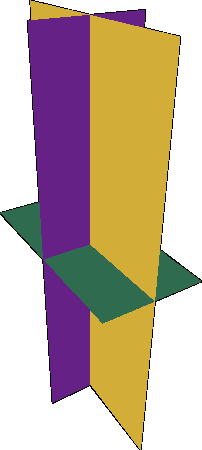
\includegraphics{asy/axesgraphic.pdf}}
  \put(9.5,-8.5){
\includegraphics{asy/shadow.pdf}}
  \put(15.25,-3){\makebox[0pt][r]{\frontcovertext{Linear Algebra}}}
  \put(15.25,-3.7){\makebox[0pt][r]{\frontcoverauthortext{Jim Hef{}feron}}}
  \put(15.25,-7.95){\makebox[0pt][r]{\frontcoverurltext{hefferon.net/linearalgebra}}}
  \put(15.25,-2.20){\makebox[0pt][r]{\frontcovereditiontext{Fourth edition}}}
  \put(7.65,-9.5){\spine}
  \put(1.0,-1.0){\backcoverhead}
  \put(1.0,-1.9){\backcovertext}

  \ifbool{showkdplinesbool}{% 
    % Front Cover width, height
    % Back cover
    \put(0.125,-0.125){\color{blue}\line(1,0){7.5}} % \FrontCoverWidth wide
      \put(0.125,-9.375){\color{blue}\line(1,0){7.5}} % \FrontCoverWidth wide
      \put(0.125,-0.125){\color{blue}\line(0,-1){9.25}} % \FrontCoverHeight tall
      \put(7.625,-0.125){\color{blue}\line(0,-1){9.25}}
    \put(0.25,-0.25){\color{blue}\line(1,0){7.375}} % \FrontCoverSafeWidth wide
      \put(0.25,-9.25){\color{blue}\line(1,0){7.375}} % \FrontCoverSafeWidth wide
      \put(0.25,-0.25){\color{blue}\line(0,-1){9.0}} % \FrontCoverSafeHeight tall
    % % Spine
    \put(7.687,-0.25){\color{blue}\line(1,0){1.071}} % 
      \put(7.687,-9.25){\color{blue}\line(1,0){1.071}} % 
    \put(7.687,-0.25){\color{blue}\line(0,-1){9}} %
      \put(8.758,-0.25){\color{blue}\line(0,-1){9}} %
    % % Front Cover
    \put(16.341,-0.125){\color{blue}\line(-1,0){7.5}} % 
      \put(16.341,-9.375){\color{blue}\line(-1,0){7.5}} % 
    \put(16.341,-0.125){\color{blue}\line(0,-1){9.25}} % 
      \put(8.821,-0.125){\color{blue}\line(0,-1){9.25}} % 
    \put(16.216,-0.25){\color{blue}\line(-1,0){7.375}} % Safe area
      \put(16.216,-9.25){\color{blue}\line(-1,0){7.375}} % 
    \put(16.216,-0.25){\color{blue}\line(0,-1){9}} % 
  }{}
\end{picture}
\end{document}
"
\ifdefined\showkdplines
  \booltrue{showkdplinesbool}
\fi
\ifbool{showkdplinesbool}{\typeout{!!! KDP LINES SHOWN}}{}

% Size of page
% Kindle Direct Publishing gives this for a 531 page book;
% see the graphic KDP_diagram_531_pages.png
% # 	Description 	Width (in) 	Height (in)
% 1 	Full Cover 	16.446 	9.5
% 2 	Front Cover 	7.5 	9.25
% 3 	Safe Area 	7.375 	9
% 4 	Bleed 	0.125 	0.125
% 5 	Margin 	0.125 	0.125
% 6 	Spine 	1.196 	9.25
% 7 	Spine Safe Area 	1.071 	9
% 8 	Spine Margin 	0.062 	0.062
% 9 	Barcode Margin 	0.25 	0.25 

% I could calculate some of these from the others, but why?
% Number 3
\newlength{\FrontCoverSafeWidth}
  \setlength{\FrontCoverSafeWidth}{7.375in}
\newlength{\FrontCoverSafeHeight}
  \setlength{\FrontCoverSafeHeight}{9in}
% Number 5
\newlength{\FrontCoverMarginWidth}
  \setlength{\FrontCoverMarginWidth}{0.125in}
\newlength{\FrontCoverMarginHeight}
  \setlength{\FrontCoverMarginHeight}{0.125in}
% Number 2
\newlength{\FrontCoverWidth}
  \setlength{\FrontCoverWidth}{7.5in}
\newlength{\FrontCoverHeight}
  \setlength{\FrontCoverHeight}{9.25in}
% Number 4
\newlength{\BleedWidth}
  \setlength{\BleedWidth}{0.125in}
\newlength{\BleedHeight}
  \setlength{\BleedHeight}{0.125in}
% Number 7
\newlength{\SpineSafeWidth}
  \setlength{\SpineSafeWidth}{1.071in}
\newlength{\SpineSafeHeight}
  \setlength{\SpineSafeHeight}{9.0in}
% Number 8
\newlength{\SpineMarginWidth}
  \setlength{\SpineMarginWidth}{0.062in}
\newlength{\SpineMarginHeight}
  \setlength{\SpineMarginHeight}{0.062in}
% Number 9
\newlength{\BarcodeMarginWidth}
  \setlength{\BarcodeMarginWidth}{0.25in}
\newlength{\BarcodeMarginHeight}
  \setlength{\BarcodeMarginHeight}{0.25in}
% Number 6
\newlength{\SpineWidth}
  \setlength{\SpineWidth}{7.375in}
\newlength{\SpineHeight}
  \setlength{\SpineHeight}{9in}
% Number 1
\newlength{\FullCoverWidth}
  \setlength{\FullCoverWidth}{16.446in}
\newlength{\FullCoverHeight}
  \setlength{\FullCoverHeight}{9.5in}

\newlength{\totalcoverwidth} \setlength{\totalcoverwidth}{15.0in} % 7.5+7.5
\newlength{\spinewidth} \setlength{\spinewidth}{1in}
\addtolength{\totalcoverwidth}{\spinewidth}
\usepackage[papersize={16.446in,10in},margin=0in]{geometry}  

% ==== Spine ========
% 
\newcommand{\spinetext}[1]{\color{black}\fontsize{38pt}{8pt}{\fontfamily{ugq}\selectfont #1}}
\newcommand{\spineauthortext}[1]{\color{coverdarkcolor}\fontsize{23pt}{8pt}{\fontfamily{ugq}\selectfont{#1}}}
\newcommand{\spine}{%
\setlength{\unitlength}{1in}
\begin{picture}(1,9.5)
  \setstackgap{S}{2.1ex}
  % \put(0.235,5.65){\Shortstack{{\spinetext{L}} {\spinetext{I}} {\spinetext{N}} {\spinetext{E}} {\spinetext{A}} {\spinetext{R}}}}
  \put(0.18,8.5){\rotatebox[origin=lc]{-90}{\spinetext{Linear Algebra}\hspace{2.15in}\spineauthortext{Hef{}feron}}}
  \setstackgap{S}{0.9ex}
  % \put(0.3925,1.15){\Shortstack{{\spineauthortext{H}{14}} {\spineauthortext{E}{14}} {\spineauthortext{F}{14}} {\spineauthortext{F}{14}} {\spineauthortext{E}{14}} {\spineauthortext{R}{14}} {\spineauthortext{O}{14}} {\spineauthortext{N}{14}}}} % tried fake small caps by making the H be 14 pt, others be 11
\end{picture}
}


% ==== Back cover ========
% 
\newcommand{\backcovertext}{%
\RaggedRight
\color{black}\fontsize{14pt}{17pt}\fontfamily{fos}\selectfont
\begin{minipage}[t]{5.75in}
\setlength{\parskip}{1.4ex}
This text covers a standard first course:
Gauss's Method, vector spaces, linear maps and matrices, determinants,
and eigenvalues and eigenvectors.
In addition, each chapter ends with some
brief topics, including applications.

What sets this book apart is careful motivation, 
many examples, and extensive exercise sets.
Together, these help each student master the material of
the course and also help an instructor develop their student's  
level of mathematical maturity.

This book
has been freely available online for many years. 
It is widely used, 
both in classrooms and for self-study.
It is supported by worked answers for all exercises, 
projection slides for classroom use, 
and a lab manual based on \textit{Sage}. 

\vspace{.2in}
\noindent\textbf{Winner of the Math Association of America's Solow Award:}\\[1.35ex]
\vspace{-.225in}
\begin{center}
\parbox{5.5in}{
``The clear writing style, tremendous variety of exercises,
amenability to use with active learning strategies, and the
careful attention to detail in preparation mean that the text
is exceptionally adaptable.''}
\end{center}
\end{minipage}
}

\newcommand{\backcoverhead}{%
\setlength{\unitlength}{1in}
\begin{picture}(0,0)
  % \put(1,-.1){{\color{coverbgcolor}\rule{4.4in}{2pt}}}
  \put(0,-.1){{\color{coverbgcolor}\rule{5.05in}{2pt}}}
  \put(0.0,0){\color{coverboldcolor}\fontsize{25pt}{8pt}\fontfamily{fos}\selectfont \textit{A developmental approach to}}
  \put(3.0,-.45){\color{black}\fontsize{25pt}{8pt}\fontfamily{fos}\selectfont \textbf{Linear Algebra}}
\end{picture}
}




% ==== Front cover ========
% 
\newcommand{\frontcovertext}[1]{\color{black}\fontsize{55pt}{8pt}{\fontfamily{ugq}\selectfont #1}}
% \newcommand{\frontcovereditiontext}[1]{\color{black}\fontsize{20pt}{8pt}{\fontfamily{ugq}\selectfont #1}}
\newcommand{\frontcovereditiontext}[1]{\color[gray]{0.4}\fontsize{20pt}{6pt}\fontfamily{ugq}\selectfont \textsf{#1}}
% \newcommand{\frontcovereditiontext}[1]{\color{black}\fontsize{20pt}{6pt}\fontfamily{ugq}\selectfont #1}
\newcommand{\frontcoverauthortext}[1]{\color{black}\fontsize{27.5pt}{6pt}{\fontfamily{ugq}\selectfont #1}}
\newcommand{\frontcoverurltext}[1]{\color[gray]{0.4}\fontsize{18pt}{6pt}\fontfamily{ugq}\selectfont \textsf{#1}}
% \newcommand{\frontcoverurltext}[1]{\color[gray]{0.4}{\lato \fontsize{18pt}{6pt}\fontseries{sb}\selectfont #1}}


\setlength{\parindent}{0in}
\begin{document}\pagestyle{empty}\thispagestyle{empty}

\setlength{\unitlength}{1in}
\begin{picture}(0,0) 
  \ifbool{showguidelinesbool}{% 
    \put(0,-1){\makebox[0in]{\color{red}0}}
    \put(1,-1){\makebox[0in]{\color{red}1}}
    \put(2,-1){\makebox[0in]{\color{red}2}}
    \put(3,-1){\makebox[0in]{\color{red}3}}
    \put(4,-1){\makebox[0in]{\color{red}4}}
    \put(5,-1){\makebox[0in]{\color{red}5}}
    \put(6,-1){\makebox[0in]{\color{red}6}}
    \put(7,-1){\makebox[0in]{\color{red}7}}
    \put(7.5,-1){\color{red}\line(0,-1){8}}
    \put(8,-1){\makebox[0in]{\color{red}8}}
    \put(8,-1){\color{blue}\line(0,-1){8}}
    \put(8.5,-1){\color{red}\line(0,-1){8}}
    \put(9,-1){\makebox[0in]{\color{red}9}}
    \put(9.5,-1){\color{blue}\line(0,-1){8}}
    \put(10,-1){\makebox[0in]{\color{red}10}}
    \put(11,-1){\makebox[0in]{\color{red}11}}
    \put(12,-1){\makebox[0in]{\color{red}12}}
    \put(13,-1){\makebox[0in]{\color{red}13}}
    \put(14,-1){\makebox[0in]{\color{red}14}}
    \put(15,-1){\makebox[0in]{\color{red}15}}
    \put(15,-1){\color{blue}\line(0,-1){8}}
    \put(16,-1){\makebox[0in]{\color{red}16}}
  }{} 

  \put(9.5,-7.57){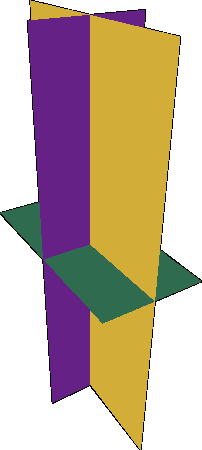
\includegraphics{asy/axesgraphic.pdf}}
  \put(9.5,-8.5){
\includegraphics{asy/shadow.pdf}}
  \put(15.25,-3){\makebox[0pt][r]{\frontcovertext{Linear Algebra}}}
  \put(15.25,-3.7){\makebox[0pt][r]{\frontcoverauthortext{Jim Hef{}feron}}}
  \put(15.25,-7.95){\makebox[0pt][r]{\frontcoverurltext{hefferon.net/linearalgebra}}}
  \put(15.25,-2.20){\makebox[0pt][r]{\frontcovereditiontext{Fourth edition}}}
  \put(7.65,-9.5){\spine}
  \put(1.0,-1.0){\backcoverhead}
  \put(1.0,-1.9){\backcovertext}

  \ifbool{showkdplinesbool}{% 
    % Front Cover width, height
    % Back cover
    \put(0.125,-0.125){\color{blue}\line(1,0){7.5}} % \FrontCoverWidth wide
      \put(0.125,-9.375){\color{blue}\line(1,0){7.5}} % \FrontCoverWidth wide
      \put(0.125,-0.125){\color{blue}\line(0,-1){9.25}} % \FrontCoverHeight tall
      \put(7.625,-0.125){\color{blue}\line(0,-1){9.25}}
    \put(0.25,-0.25){\color{blue}\line(1,0){7.375}} % \FrontCoverSafeWidth wide
      \put(0.25,-9.25){\color{blue}\line(1,0){7.375}} % \FrontCoverSafeWidth wide
      \put(0.25,-0.25){\color{blue}\line(0,-1){9.0}} % \FrontCoverSafeHeight tall
    % % Spine
    \put(7.687,-0.25){\color{blue}\line(1,0){1.071}} % 
      \put(7.687,-9.25){\color{blue}\line(1,0){1.071}} % 
    \put(7.687,-0.25){\color{blue}\line(0,-1){9}} %
      \put(8.758,-0.25){\color{blue}\line(0,-1){9}} %
    % % Front Cover
    \put(16.341,-0.125){\color{blue}\line(-1,0){7.5}} % 
      \put(16.341,-9.375){\color{blue}\line(-1,0){7.5}} % 
    \put(16.341,-0.125){\color{blue}\line(0,-1){9.25}} % 
      \put(8.821,-0.125){\color{blue}\line(0,-1){9.25}} % 
    \put(16.216,-0.25){\color{blue}\line(-1,0){7.375}} % Safe area
      \put(16.216,-9.25){\color{blue}\line(-1,0){7.375}} % 
    \put(16.216,-0.25){\color{blue}\line(0,-1){9}} % 
  }{}
\end{picture}
\end{document}
"
\ifdefined\showkdplines
  \booltrue{showkdplinesbool}
\fi
\ifbool{showkdplinesbool}{\typeout{!!! KDP LINES SHOWN}}{}

% Size of page
% Kindle Direct Publishing gives this for a 531 page book;
% see the graphic KDP_diagram_531_pages.png
% # 	Description 	Width (in) 	Height (in)
% 1 	Full Cover 	16.446 	9.5
% 2 	Front Cover 	7.5 	9.25
% 3 	Safe Area 	7.375 	9
% 4 	Bleed 	0.125 	0.125
% 5 	Margin 	0.125 	0.125
% 6 	Spine 	1.196 	9.25
% 7 	Spine Safe Area 	1.071 	9
% 8 	Spine Margin 	0.062 	0.062
% 9 	Barcode Margin 	0.25 	0.25 

% I could calculate some of these from the others, but why?
% Number 3
\newlength{\FrontCoverSafeWidth}
  \setlength{\FrontCoverSafeWidth}{7.375in}
\newlength{\FrontCoverSafeHeight}
  \setlength{\FrontCoverSafeHeight}{9in}
% Number 5
\newlength{\FrontCoverMarginWidth}
  \setlength{\FrontCoverMarginWidth}{0.125in}
\newlength{\FrontCoverMarginHeight}
  \setlength{\FrontCoverMarginHeight}{0.125in}
% Number 2
\newlength{\FrontCoverWidth}
  \setlength{\FrontCoverWidth}{7.5in}
\newlength{\FrontCoverHeight}
  \setlength{\FrontCoverHeight}{9.25in}
% Number 4
\newlength{\BleedWidth}
  \setlength{\BleedWidth}{0.125in}
\newlength{\BleedHeight}
  \setlength{\BleedHeight}{0.125in}
% Number 7
\newlength{\SpineSafeWidth}
  \setlength{\SpineSafeWidth}{1.071in}
\newlength{\SpineSafeHeight}
  \setlength{\SpineSafeHeight}{9.0in}
% Number 8
\newlength{\SpineMarginWidth}
  \setlength{\SpineMarginWidth}{0.062in}
\newlength{\SpineMarginHeight}
  \setlength{\SpineMarginHeight}{0.062in}
% Number 9
\newlength{\BarcodeMarginWidth}
  \setlength{\BarcodeMarginWidth}{0.25in}
\newlength{\BarcodeMarginHeight}
  \setlength{\BarcodeMarginHeight}{0.25in}
% Number 6
\newlength{\SpineWidth}
  \setlength{\SpineWidth}{7.375in}
\newlength{\SpineHeight}
  \setlength{\SpineHeight}{9in}
% Number 1
\newlength{\FullCoverWidth}
  \setlength{\FullCoverWidth}{16.446in}
\newlength{\FullCoverHeight}
  \setlength{\FullCoverHeight}{9.5in}

\newlength{\totalcoverwidth} \setlength{\totalcoverwidth}{15.0in} % 7.5+7.5
\newlength{\spinewidth} \setlength{\spinewidth}{1in}
\addtolength{\totalcoverwidth}{\spinewidth}
\usepackage[papersize={16.446in,10in},margin=0in]{geometry}  

% ==== Spine ========
% 
\newcommand{\spinetext}[1]{\color{black}\fontsize{38pt}{8pt}{\fontfamily{ugq}\selectfont #1}}
\newcommand{\spineauthortext}[1]{\color{coverdarkcolor}\fontsize{23pt}{8pt}{\fontfamily{ugq}\selectfont{#1}}}
\newcommand{\spine}{%
\setlength{\unitlength}{1in}
\begin{picture}(1,9.5)
  \setstackgap{S}{2.1ex}
  % \put(0.235,5.65){\Shortstack{{\spinetext{L}} {\spinetext{I}} {\spinetext{N}} {\spinetext{E}} {\spinetext{A}} {\spinetext{R}}}}
  \put(0.18,8.5){\rotatebox[origin=lc]{-90}{\spinetext{Linear Algebra}\hspace{2.15in}\spineauthortext{Hef{}feron}}}
  \setstackgap{S}{0.9ex}
  % \put(0.3925,1.15){\Shortstack{{\spineauthortext{H}{14}} {\spineauthortext{E}{14}} {\spineauthortext{F}{14}} {\spineauthortext{F}{14}} {\spineauthortext{E}{14}} {\spineauthortext{R}{14}} {\spineauthortext{O}{14}} {\spineauthortext{N}{14}}}} % tried fake small caps by making the H be 14 pt, others be 11
\end{picture}
}


% ==== Back cover ========
% 
\newcommand{\backcovertext}{%
\RaggedRight
\color{black}\fontsize{14pt}{17pt}\fontfamily{fos}\selectfont
\begin{minipage}[t]{5.75in}
\setlength{\parskip}{1.4ex}
This text covers a standard first course:
Gauss's Method, vector spaces, linear maps and matrices, determinants,
and eigenvalues and eigenvectors.
In addition, each chapter ends with some
brief topics, including applications.

What sets this book apart is careful motivation, 
many examples, and extensive exercise sets.
Together, these help each student master the material of
the course and also help an instructor develop their student's  
level of mathematical maturity.

This book
has been freely available online for many years. 
It is widely used, 
both in classrooms and for self-study.
It is supported by worked answers for all exercises, 
projection slides for classroom use, 
and a lab manual based on \textit{Sage}. 

\vspace{.2in}
\noindent\textbf{Winner of the Math Association of America's Solow Award:}\\[1.35ex]
\vspace{-.225in}
\begin{center}
\parbox{5.5in}{
``The clear writing style, tremendous variety of exercises,
amenability to use with active learning strategies, and the
careful attention to detail in preparation mean that the text
is exceptionally adaptable.''}
\end{center}
\end{minipage}
}

\newcommand{\backcoverhead}{%
\setlength{\unitlength}{1in}
\begin{picture}(0,0)
  % \put(1,-.1){{\color{coverbgcolor}\rule{4.4in}{2pt}}}
  \put(0,-.1){{\color{coverbgcolor}\rule{5.05in}{2pt}}}
  \put(0.0,0){\color{coverboldcolor}\fontsize{25pt}{8pt}\fontfamily{fos}\selectfont \textit{A developmental approach to}}
  \put(3.0,-.45){\color{black}\fontsize{25pt}{8pt}\fontfamily{fos}\selectfont \textbf{Linear Algebra}}
\end{picture}
}




% ==== Front cover ========
% 
\newcommand{\frontcovertext}[1]{\color{black}\fontsize{55pt}{8pt}{\fontfamily{ugq}\selectfont #1}}
% \newcommand{\frontcovereditiontext}[1]{\color{black}\fontsize{20pt}{8pt}{\fontfamily{ugq}\selectfont #1}}
\newcommand{\frontcovereditiontext}[1]{\color[gray]{0.4}\fontsize{20pt}{6pt}\fontfamily{ugq}\selectfont \textsf{#1}}
% \newcommand{\frontcovereditiontext}[1]{\color{black}\fontsize{20pt}{6pt}\fontfamily{ugq}\selectfont #1}
\newcommand{\frontcoverauthortext}[1]{\color{black}\fontsize{27.5pt}{6pt}{\fontfamily{ugq}\selectfont #1}}
\newcommand{\frontcoverurltext}[1]{\color[gray]{0.4}\fontsize{18pt}{6pt}\fontfamily{ugq}\selectfont \textsf{#1}}
% \newcommand{\frontcoverurltext}[1]{\color[gray]{0.4}{\lato \fontsize{18pt}{6pt}\fontseries{sb}\selectfont #1}}


\setlength{\parindent}{0in}
\begin{document}\pagestyle{empty}\thispagestyle{empty}

\setlength{\unitlength}{1in}
\begin{picture}(0,0) 
  \ifbool{showguidelinesbool}{% 
    \put(0,-1){\makebox[0in]{\color{red}0}}
    \put(1,-1){\makebox[0in]{\color{red}1}}
    \put(2,-1){\makebox[0in]{\color{red}2}}
    \put(3,-1){\makebox[0in]{\color{red}3}}
    \put(4,-1){\makebox[0in]{\color{red}4}}
    \put(5,-1){\makebox[0in]{\color{red}5}}
    \put(6,-1){\makebox[0in]{\color{red}6}}
    \put(7,-1){\makebox[0in]{\color{red}7}}
    \put(7.5,-1){\color{red}\line(0,-1){8}}
    \put(8,-1){\makebox[0in]{\color{red}8}}
    \put(8,-1){\color{blue}\line(0,-1){8}}
    \put(8.5,-1){\color{red}\line(0,-1){8}}
    \put(9,-1){\makebox[0in]{\color{red}9}}
    \put(9.5,-1){\color{blue}\line(0,-1){8}}
    \put(10,-1){\makebox[0in]{\color{red}10}}
    \put(11,-1){\makebox[0in]{\color{red}11}}
    \put(12,-1){\makebox[0in]{\color{red}12}}
    \put(13,-1){\makebox[0in]{\color{red}13}}
    \put(14,-1){\makebox[0in]{\color{red}14}}
    \put(15,-1){\makebox[0in]{\color{red}15}}
    \put(15,-1){\color{blue}\line(0,-1){8}}
    \put(16,-1){\makebox[0in]{\color{red}16}}
  }{} 

  \put(9.5,-7.57){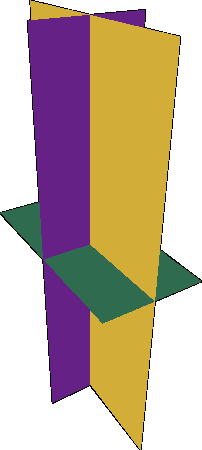
\includegraphics{asy/axesgraphic.pdf}}
  \put(9.5,-8.5){
\includegraphics{asy/shadow.pdf}}
  \put(15.25,-3){\makebox[0pt][r]{\frontcovertext{Linear Algebra}}}
  \put(15.25,-3.7){\makebox[0pt][r]{\frontcoverauthortext{Jim Hef{}feron}}}
  \put(15.25,-7.95){\makebox[0pt][r]{\frontcoverurltext{hefferon.net/linearalgebra}}}
  \put(15.25,-2.20){\makebox[0pt][r]{\frontcovereditiontext{Fourth edition}}}
  \put(7.65,-9.5){\spine}
  \put(1.0,-1.0){\backcoverhead}
  \put(1.0,-1.9){\backcovertext}

  \ifbool{showkdplinesbool}{% 
    % Front Cover width, height
    % Back cover
    \put(0.125,-0.125){\color{blue}\line(1,0){7.5}} % \FrontCoverWidth wide
      \put(0.125,-9.375){\color{blue}\line(1,0){7.5}} % \FrontCoverWidth wide
      \put(0.125,-0.125){\color{blue}\line(0,-1){9.25}} % \FrontCoverHeight tall
      \put(7.625,-0.125){\color{blue}\line(0,-1){9.25}}
    \put(0.25,-0.25){\color{blue}\line(1,0){7.375}} % \FrontCoverSafeWidth wide
      \put(0.25,-9.25){\color{blue}\line(1,0){7.375}} % \FrontCoverSafeWidth wide
      \put(0.25,-0.25){\color{blue}\line(0,-1){9.0}} % \FrontCoverSafeHeight tall
    % % Spine
    \put(7.687,-0.25){\color{blue}\line(1,0){1.071}} % 
      \put(7.687,-9.25){\color{blue}\line(1,0){1.071}} % 
    \put(7.687,-0.25){\color{blue}\line(0,-1){9}} %
      \put(8.758,-0.25){\color{blue}\line(0,-1){9}} %
    % % Front Cover
    \put(16.341,-0.125){\color{blue}\line(-1,0){7.5}} % 
      \put(16.341,-9.375){\color{blue}\line(-1,0){7.5}} % 
    \put(16.341,-0.125){\color{blue}\line(0,-1){9.25}} % 
      \put(8.821,-0.125){\color{blue}\line(0,-1){9.25}} % 
    \put(16.216,-0.25){\color{blue}\line(-1,0){7.375}} % Safe area
      \put(16.216,-9.25){\color{blue}\line(-1,0){7.375}} % 
    \put(16.216,-0.25){\color{blue}\line(0,-1){9}} % 
  }{}
\end{picture}
\end{document}
